\chapter{Methodology}

The research questions are addressed via an exploratory study involving Flemish architecture offices. The methodology is outlined in five sequential stages (figure \ref{fig:methodologycasestudy}):

% DMOA (\href{https://www.dmoa.be/}{dmoa.be}) and LAVA (\href{https://lava-architecten.be/}{lava-architecten.be}). \\

\begin{itemize}
    \item Semi-structured \textbf{interviews} with one partner from each office, to identify and agree upon the specific mannerisms to be trained on (section \ref{sec:Interviews});
    \item \textbf{Collecting} training datasets of images (section \ref{sec:Finalized training datasets});
    \item \textbf{verifying} those images with the architects (section \ref{sec:Finalized training datasets});
    \item \textbf{Training} LoRAs on these datasets (the methodology for training the LoRAs is explained in section \ref{sec:LoRA training methodology});
    \item \textbf{Evaluating} the resulting LoRAs in two settings: a controlled design process and a freer application. (section \ref{sec:Evaluation sessions})
\end{itemize}
\begin{figure}[H]
    \centering
    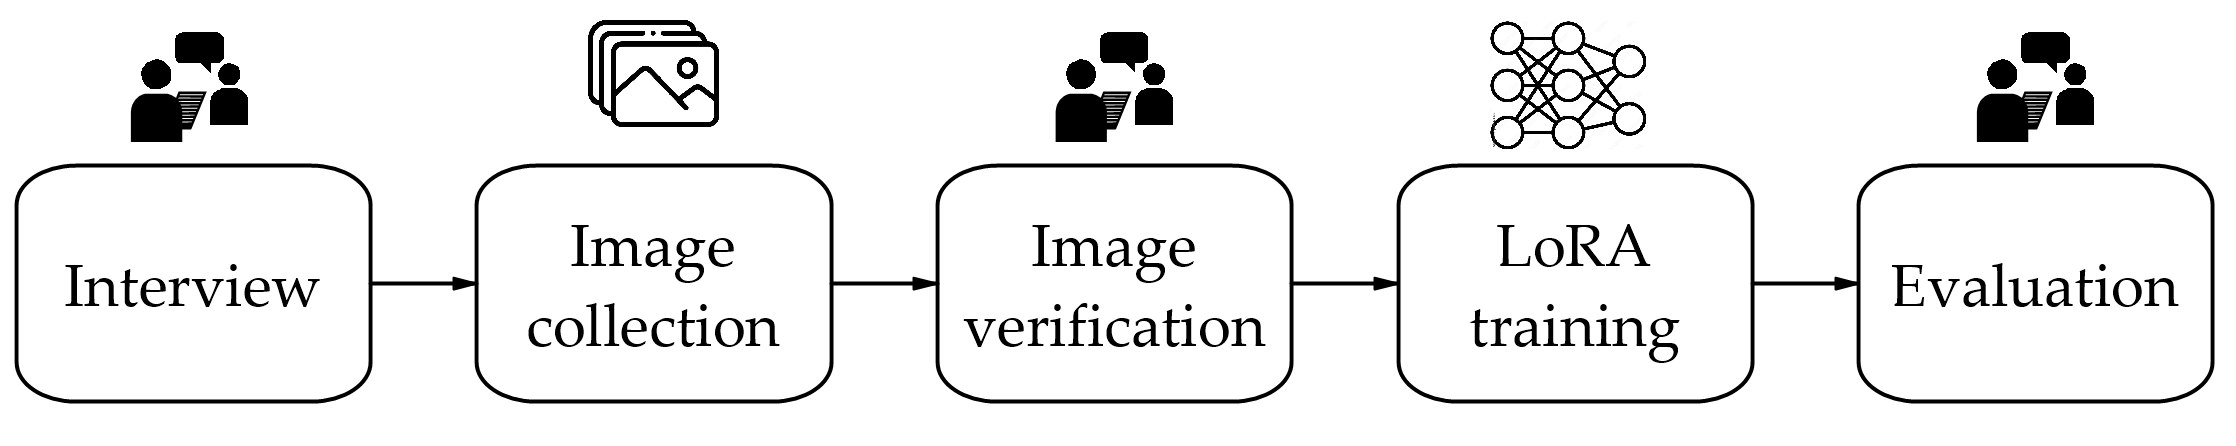
\includegraphics[width=\linewidth]{Images/Methodology/Methodology.jpg}
    \caption{The methodology of the case study.}
    \label{fig:methodologycasestudy}
\end{figure}

\section{Interviews} \label{sec:Interviews}

The selection of the mannerisms was based on semi-structured interviews with the architects (one partner from DMOA and one partner from LAVA). Based on these interviews, six mannerisms (3 per architect) were selected to align with the architects' preferences and expectations.\\ The interviews covered personal style, the role of mannerisms in their design, and prospective uses of LoRA in their design process, after which candidate mannerisms were proposed, based on review of the architects' projects and own expertise on training LoRAs. The architects then selected the 3 mannerisms they thought most useful.

\section{Image selection and verification} \label{sec:Finalized training datasets}
LoRA training requires a diverse collection of high-quality images that capture the concept in diverse environments, lightings and camera angles (\cite{deepfates_fine-tune_2024}).\\
To ensure equal influence on the model, all images were resized to 1024 x 1024 px using the online image resizer BIRME (https://www.birme.net/), matching the default output format for FLUX.1. The end result of the collection phase was a selection of 15-19 images for each LoRA.\\~\\
Prior to LoRA training, both architects reviewed the selected images through a google form, rating each image from 1 (poor representation of the concept) to 3 (clear representation). After a brief online call where the architects clarified their intentions, the image set was revised: certain images were removed and new ones added to better reflect the concept. The newly added images were not reviewed by the architects: it was assumed that the discussion had provided sufficient understanding of the architects' vision to select appropriate images.
\subsection{Finalized datasets for DMOA}
\subsubsection{Stampbeton}
The first LoRA trained for the office of DMOA is meant to replicate the material stamped concrete ('stampbeton' in Dutch). The architects have developed and patented a specific mixture of materials to create their version of the material.\\
% To train this LoRA, several images were used of two projects by DMOA: Farmer's House and KRUUL. Next to that, images of Peter Zumthor's Bruder Klaus Field Chapel in Mechernich, Germany, as well as an interior application of the material were used.\\
After validation, one image (figure \ref{fig:stampbetonomittedimage}) was left out of the original dataset: the dirty spots on the concrete in the image were too prominent, and the concrete did not sufficiently represent the typical horizontal layering of stamped concrete.
\begin{figure}[H]
    \centering
    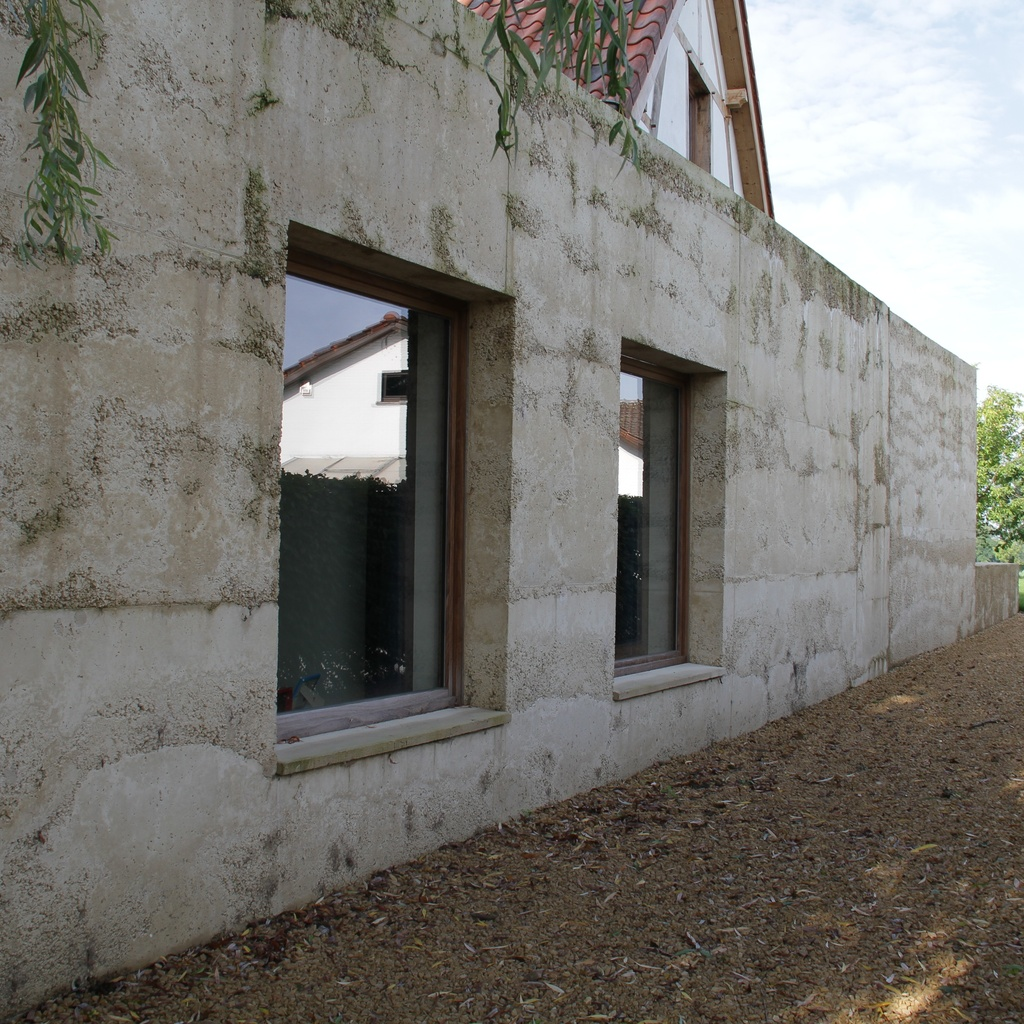
\includegraphics[width=0.24\linewidth]{Images//LoRAs//STAMPBETON/12.jpg}
    \caption{The image removed from the original dataset.}
    \label{fig:stampbetonomittedimage}
\end{figure}
Figure \ref{fig:gridstampbeton} portrays the training images for this LoRA.
\newcommand{\cellwidth}{0.24\textwidth}
\begin{figure}[H]
  \centering
  \resizebox{\textwidth}{!}{%
    \begin{tabular}{@{}ccccc@{}}
      % Row 1: images 1–5
      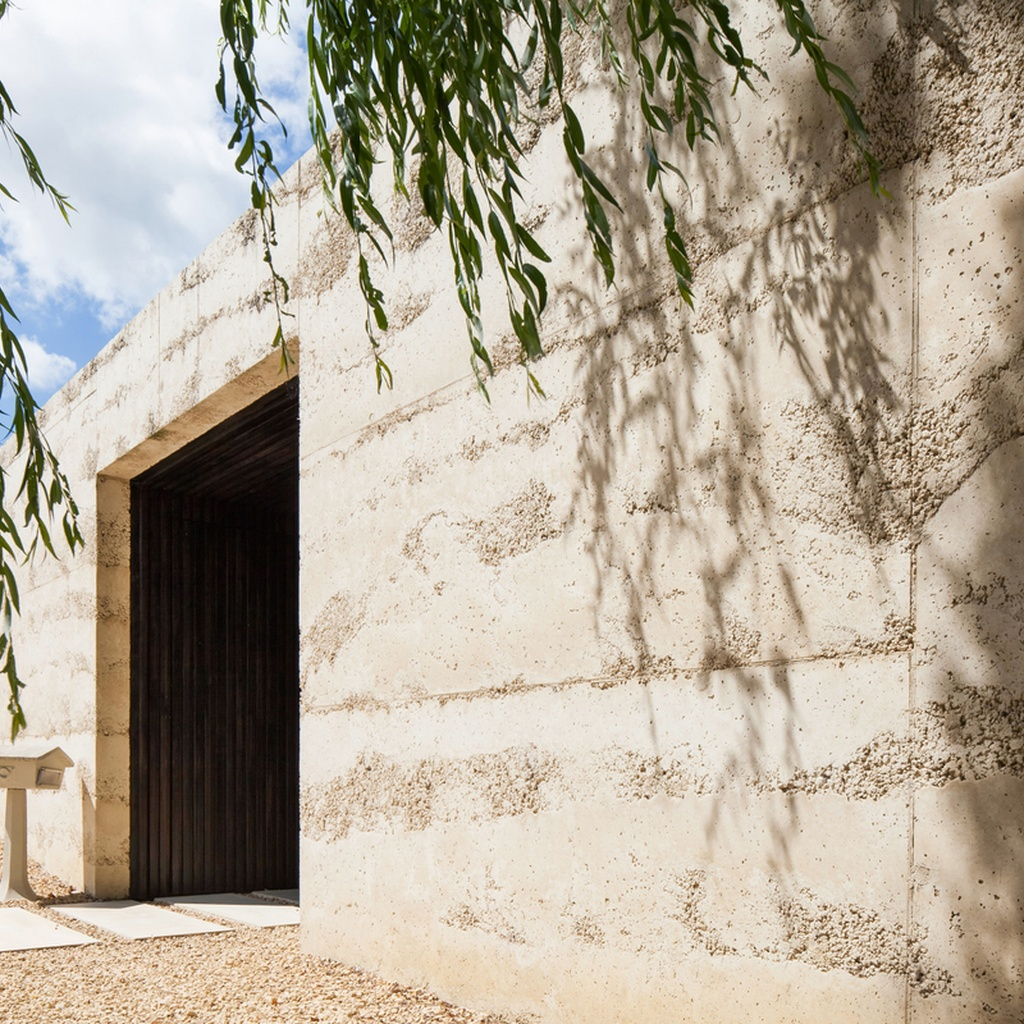
\includegraphics[width=\linewidth]{Images/LoRAs/STAMPBETON/Training_images/1.jpg} &
      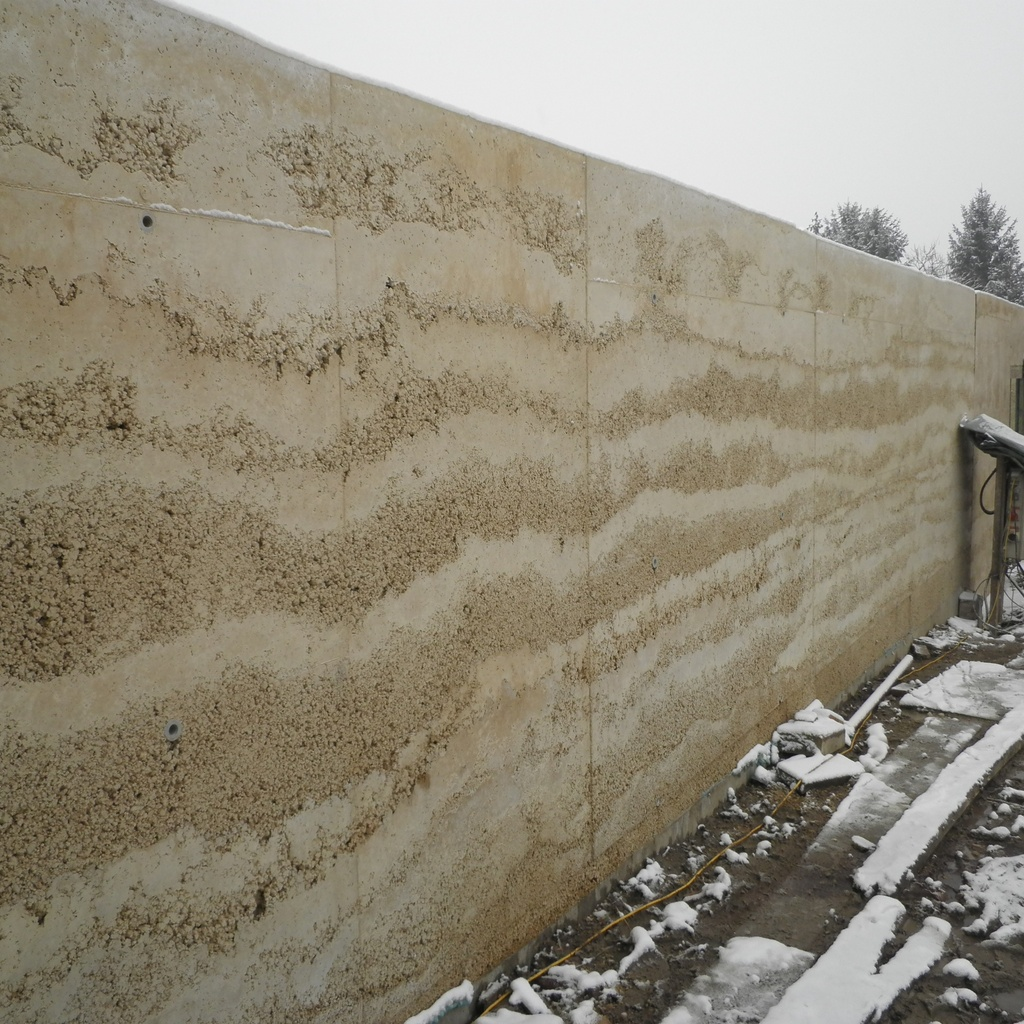
\includegraphics[width=\linewidth]{Images/LoRAs/STAMPBETON/Training_images/2.jpg} &
      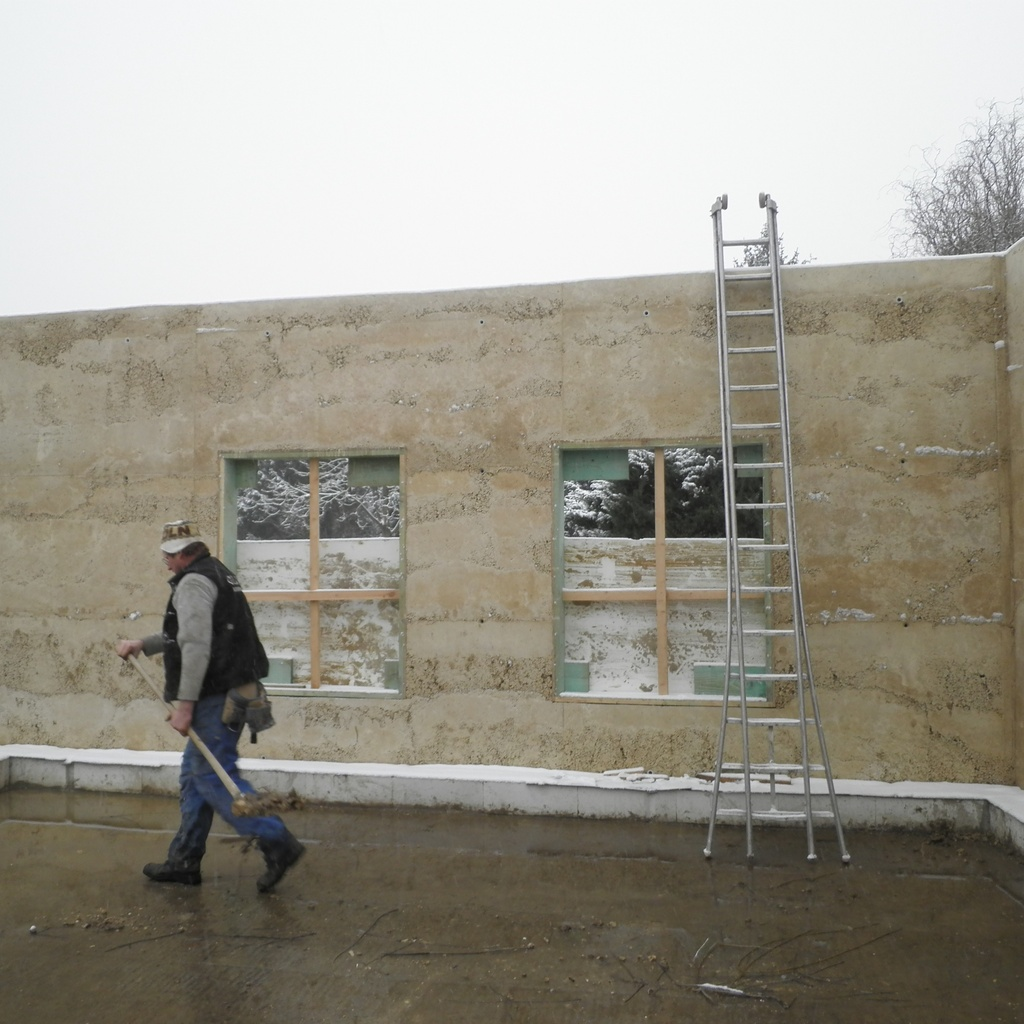
\includegraphics[width=\linewidth]{Images/LoRAs/STAMPBETON/Training_images/3.jpg} &
      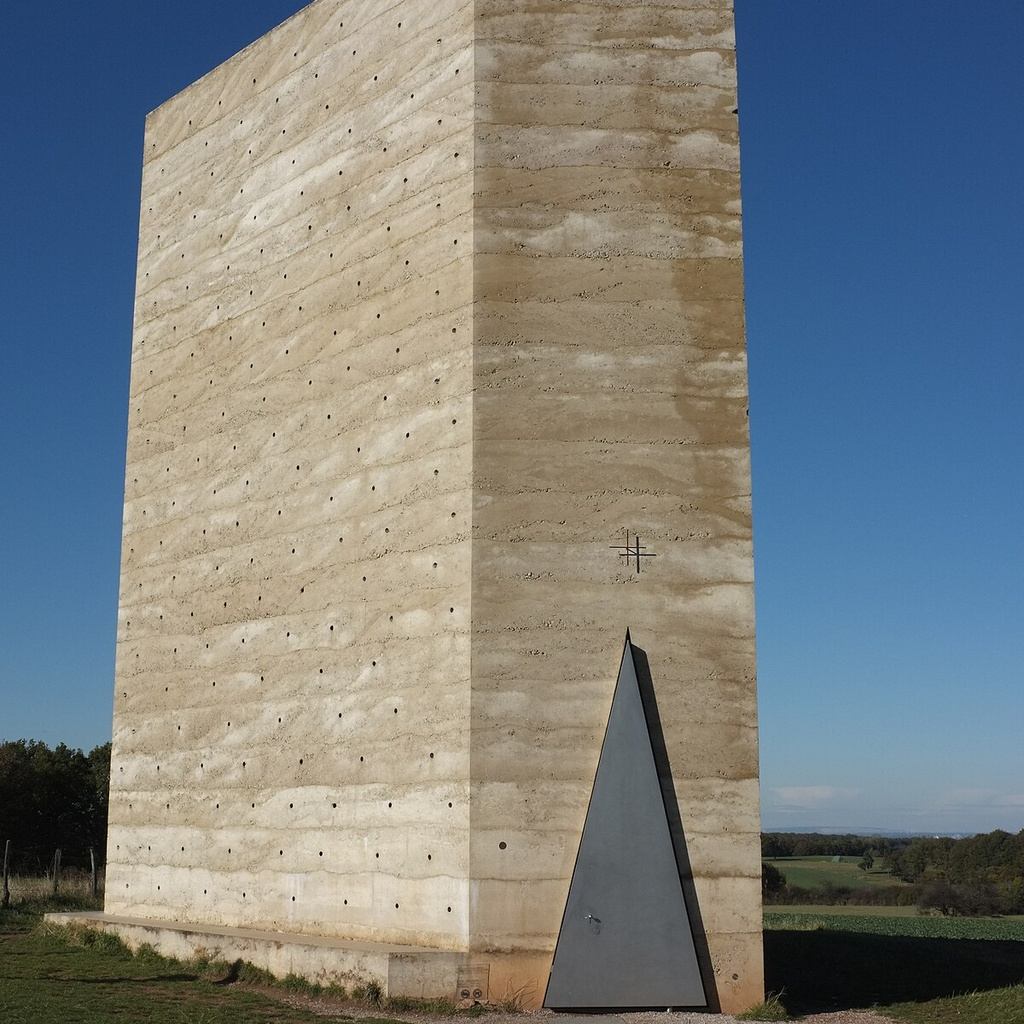
\includegraphics[width=\linewidth]{Images/LoRAs/STAMPBETON/Training_images/4.jpg} &
      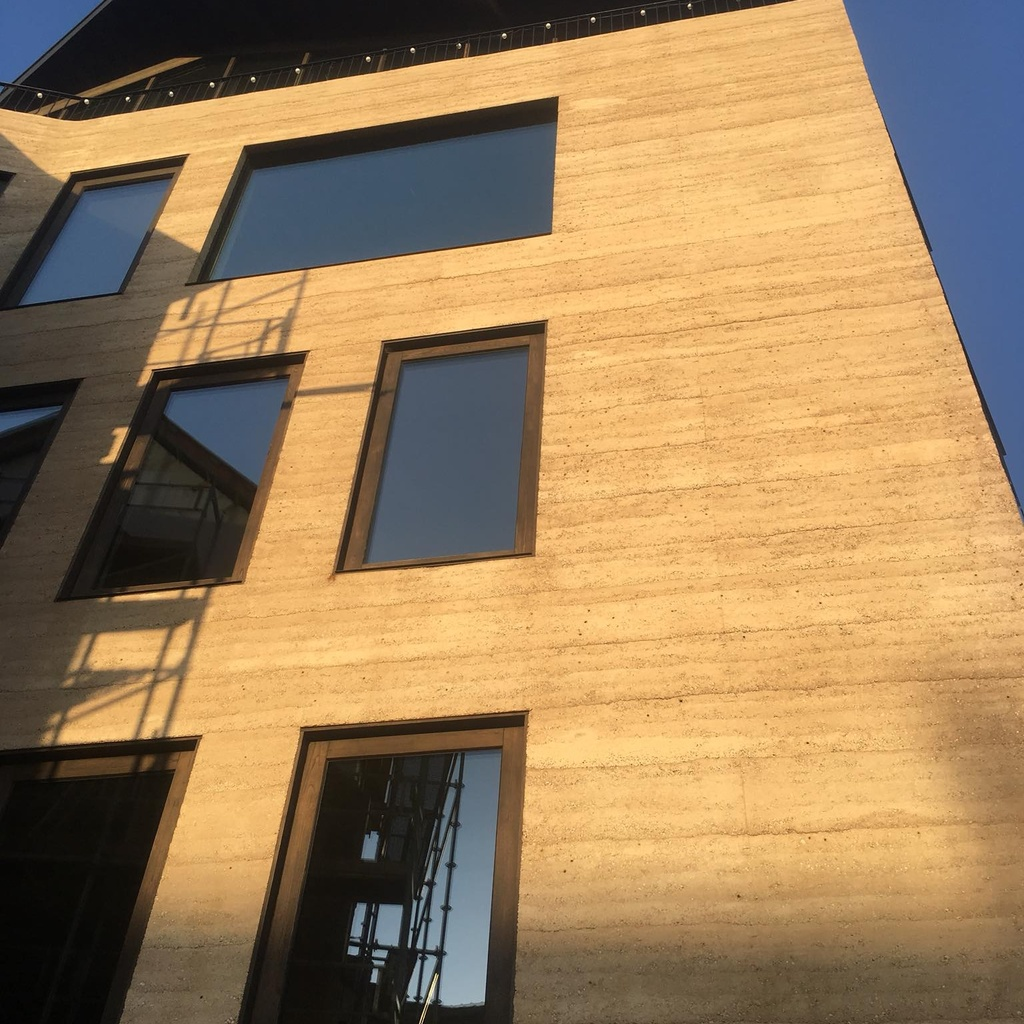
\includegraphics[width=\linewidth]{Images/LoRAs/STAMPBETON/Training_images/5.jpg} \\[2pt]

      % Row 2: images 6–10
      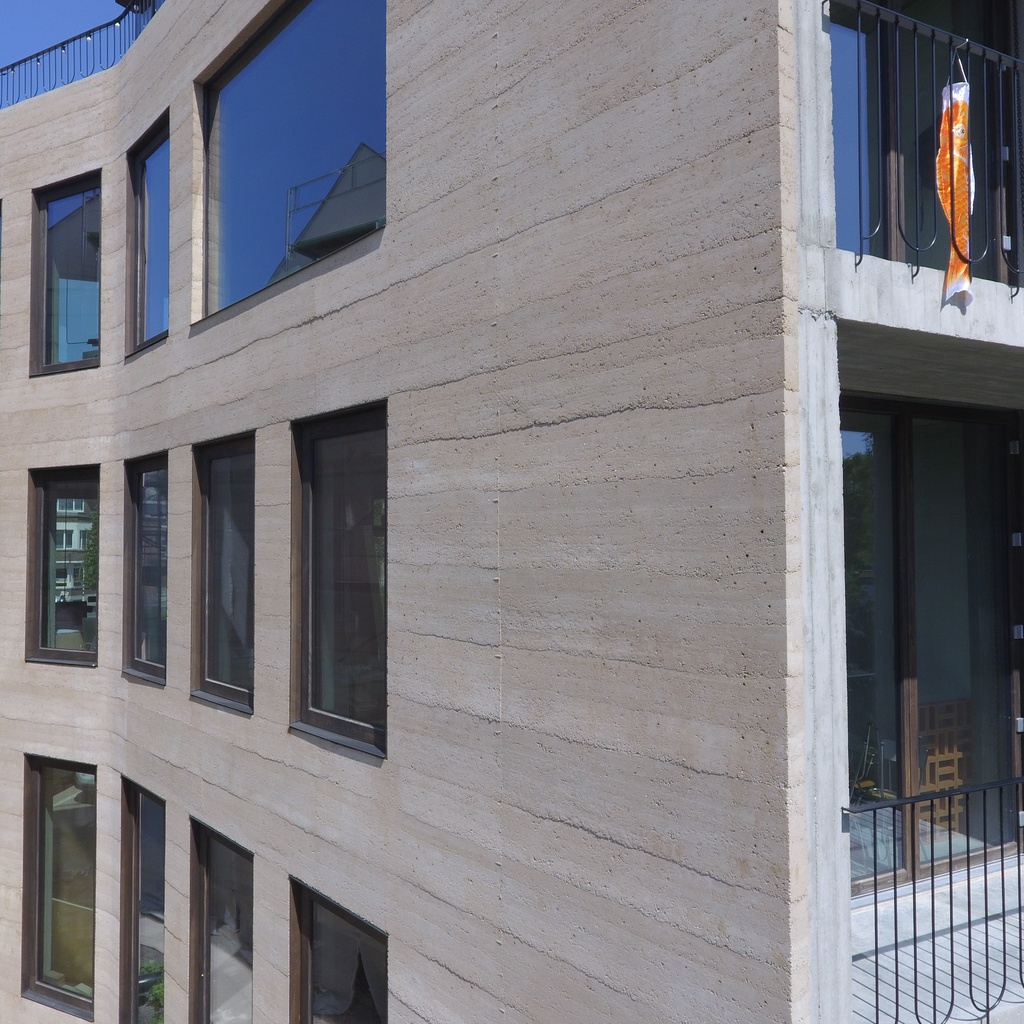
\includegraphics[width=\linewidth]{Images/LoRAs/STAMPBETON/Training_images/6.jpg} &
      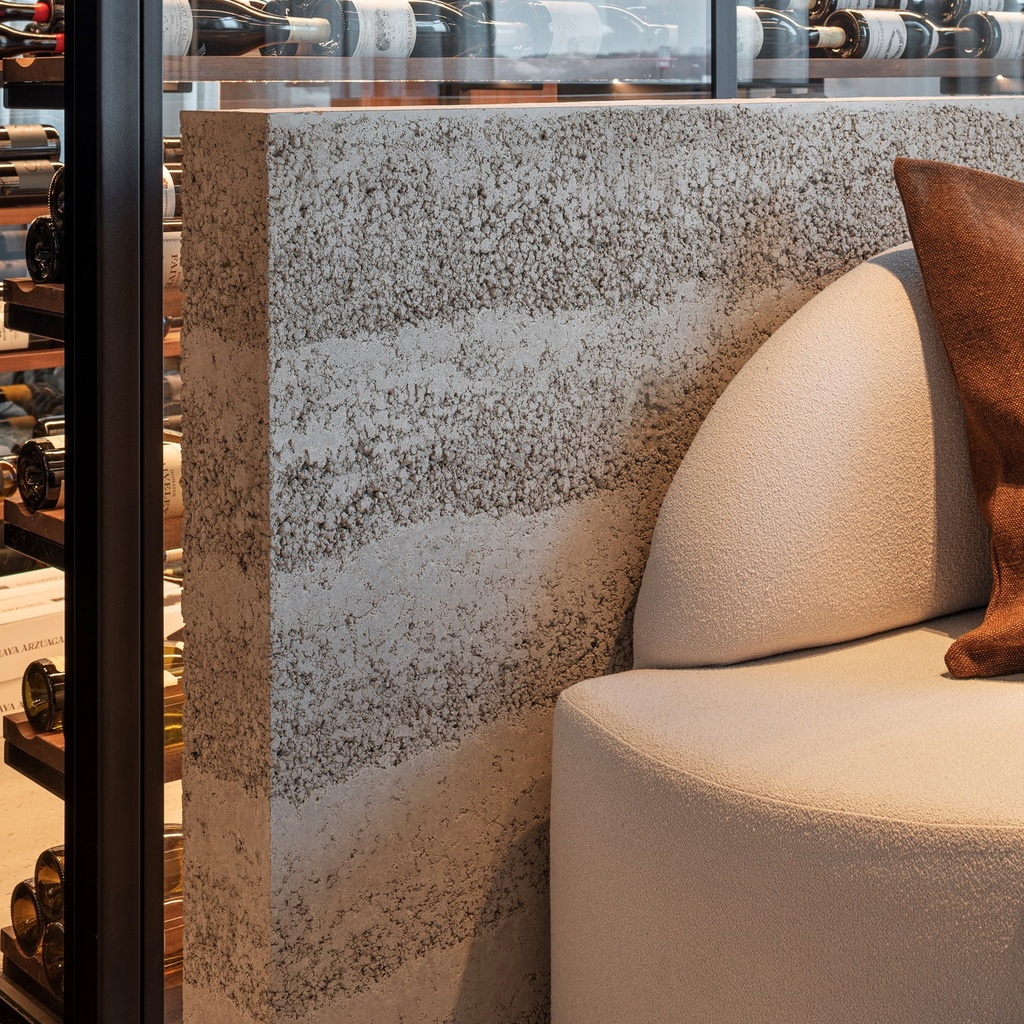
\includegraphics[width=\linewidth]{Images/LoRAs/STAMPBETON/Training_images/7.jpg} &
      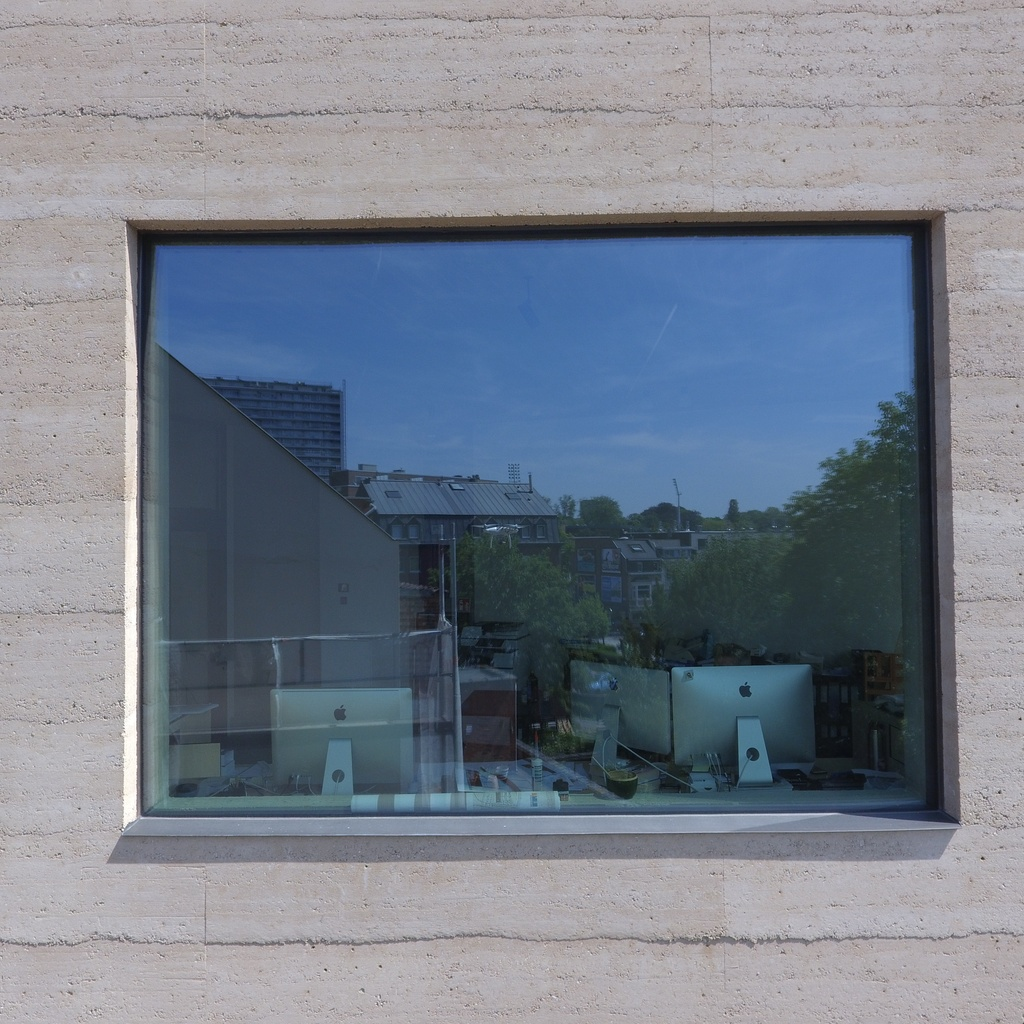
\includegraphics[width=\linewidth]{Images/LoRAs/STAMPBETON/Training_images/8.jpg} &
      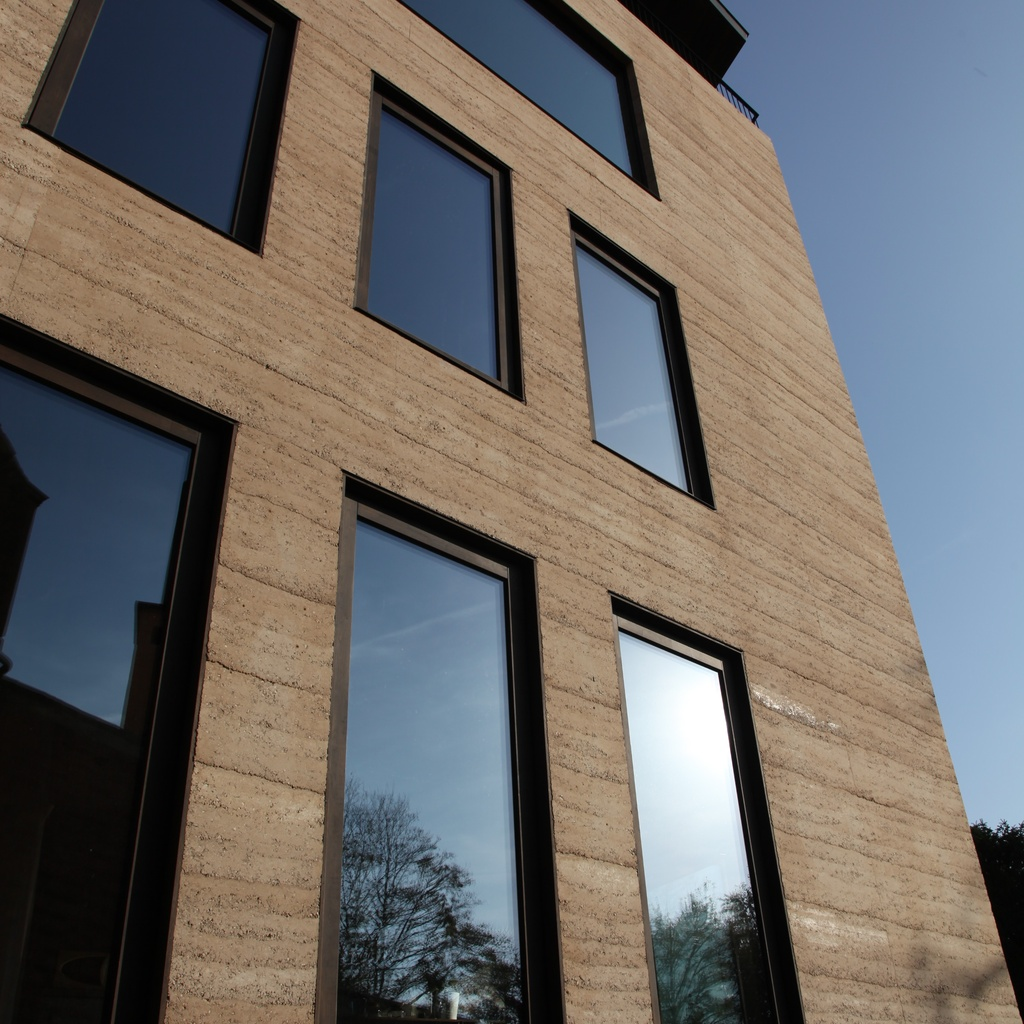
\includegraphics[width=\linewidth]{Images/LoRAs/STAMPBETON/Training_images/9.jpg} &
      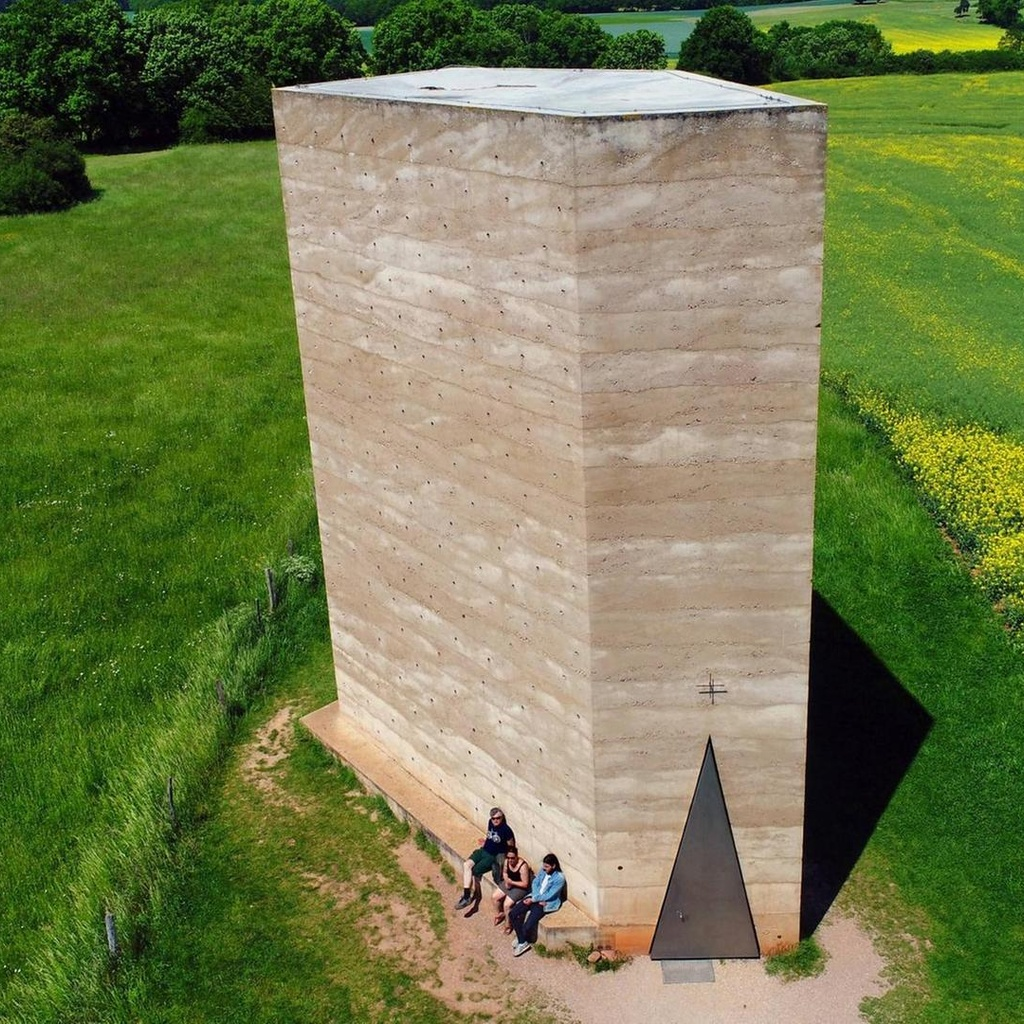
\includegraphics[width=\linewidth]{Images/LoRAs/STAMPBETON/Training_images/10.jpg} \\[2pt]

      % Row 3: images 11–15
      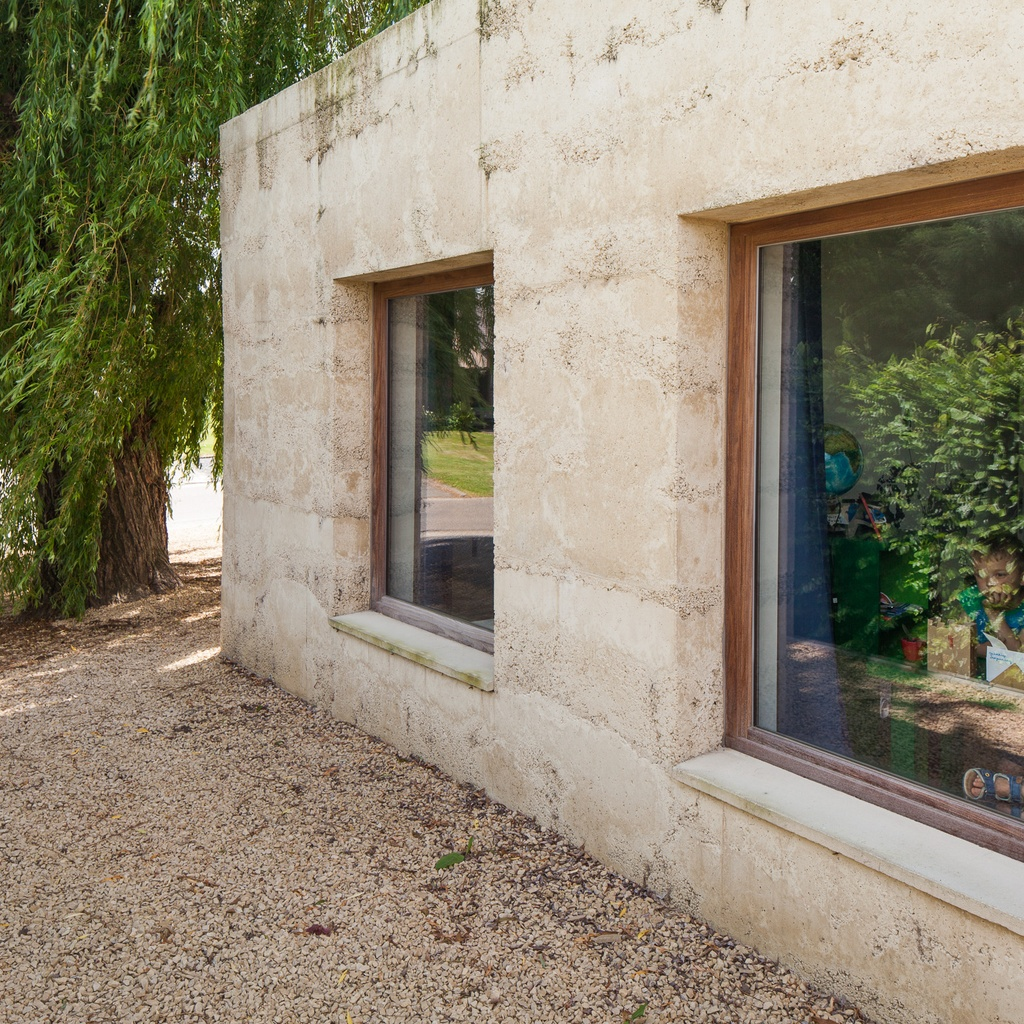
\includegraphics[width=\linewidth]{Images/LoRAs/STAMPBETON/Training_images/11.jpg} &
      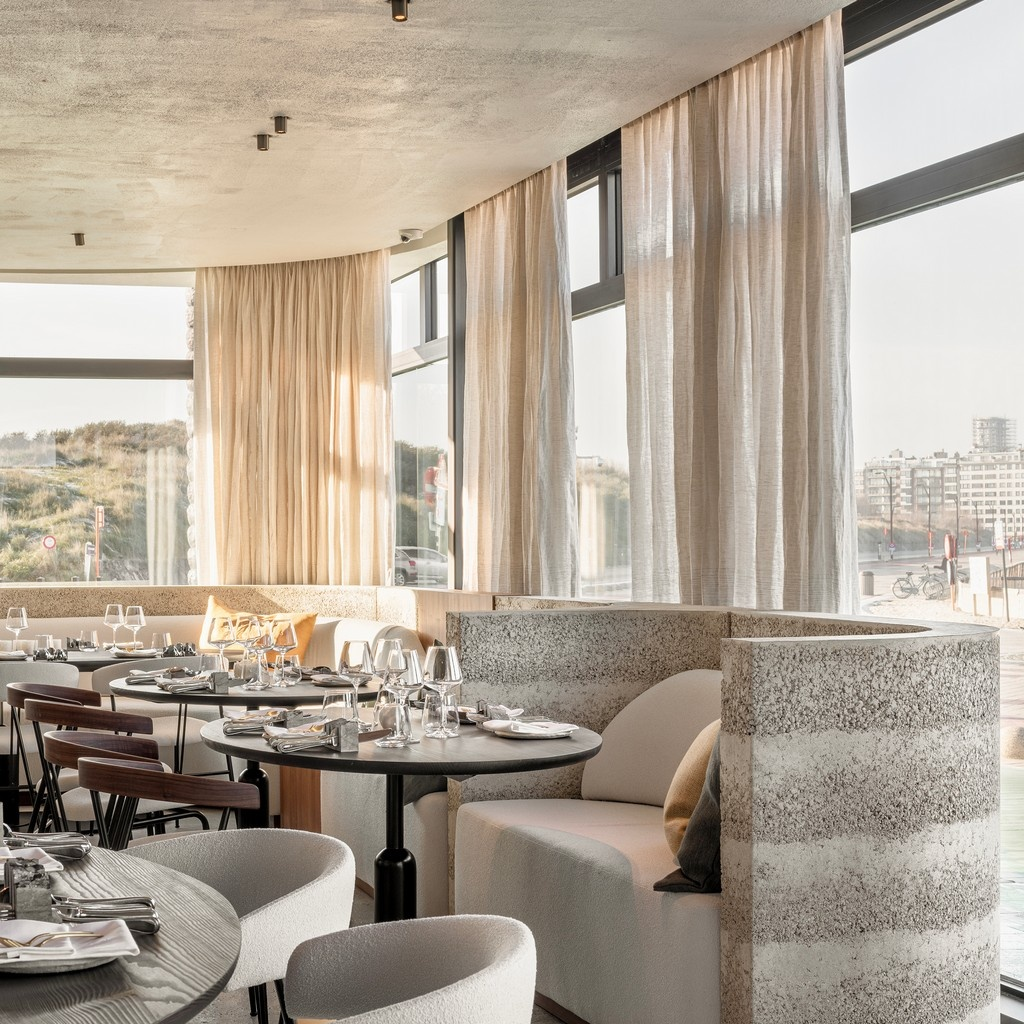
\includegraphics[width=\linewidth]{Images/LoRAs/STAMPBETON/Training_images/12.jpg} &
      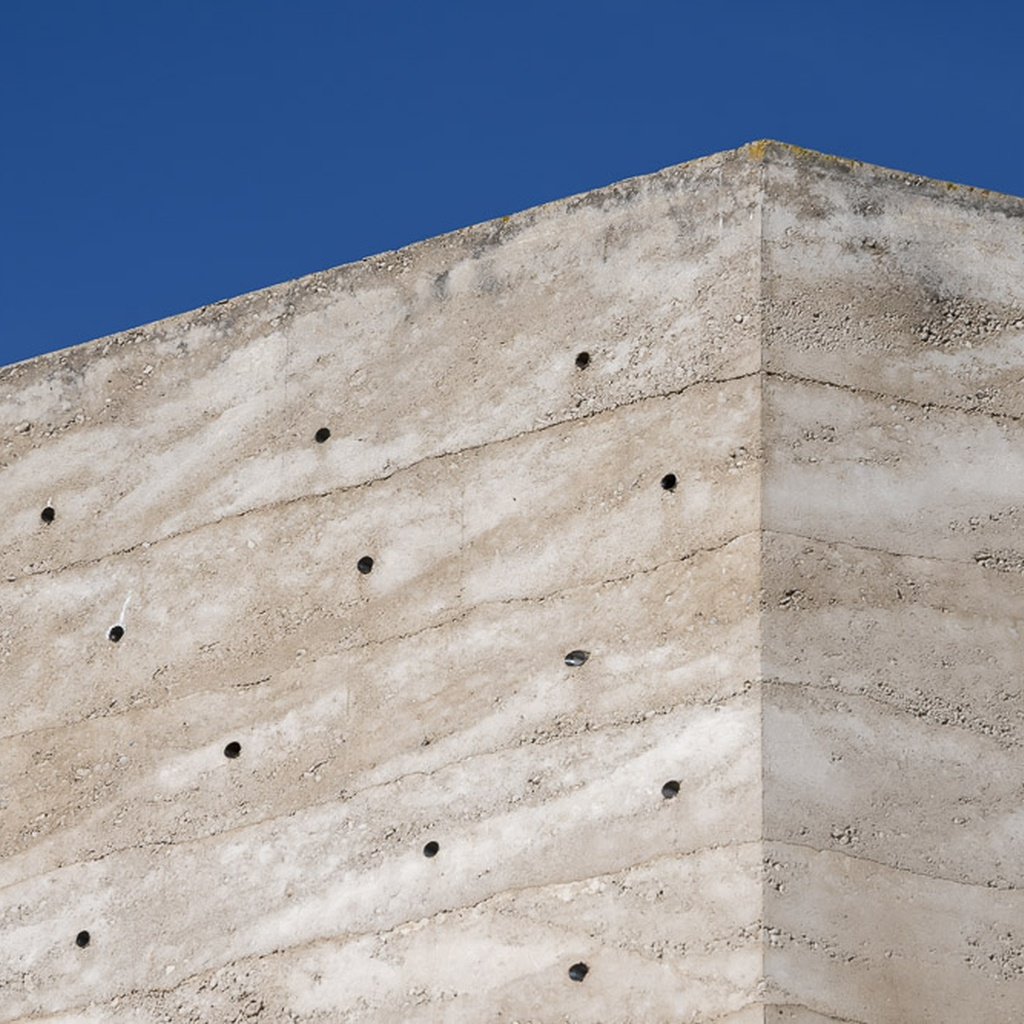
\includegraphics[width=\linewidth]{Images/LoRAs/STAMPBETON/Training_images/13.jpg} &
      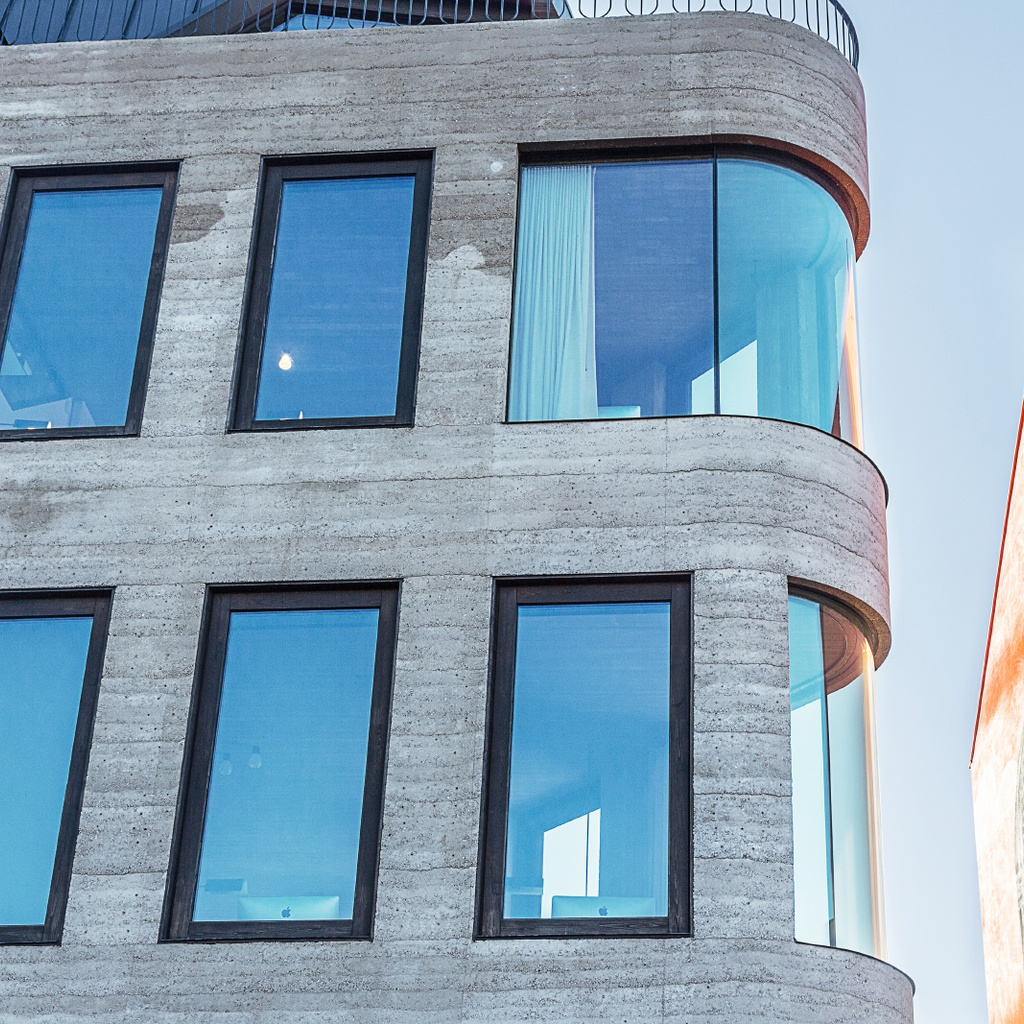
\includegraphics[width=\linewidth]{Images/LoRAs/STAMPBETON/Training_images/14.jpg} &
      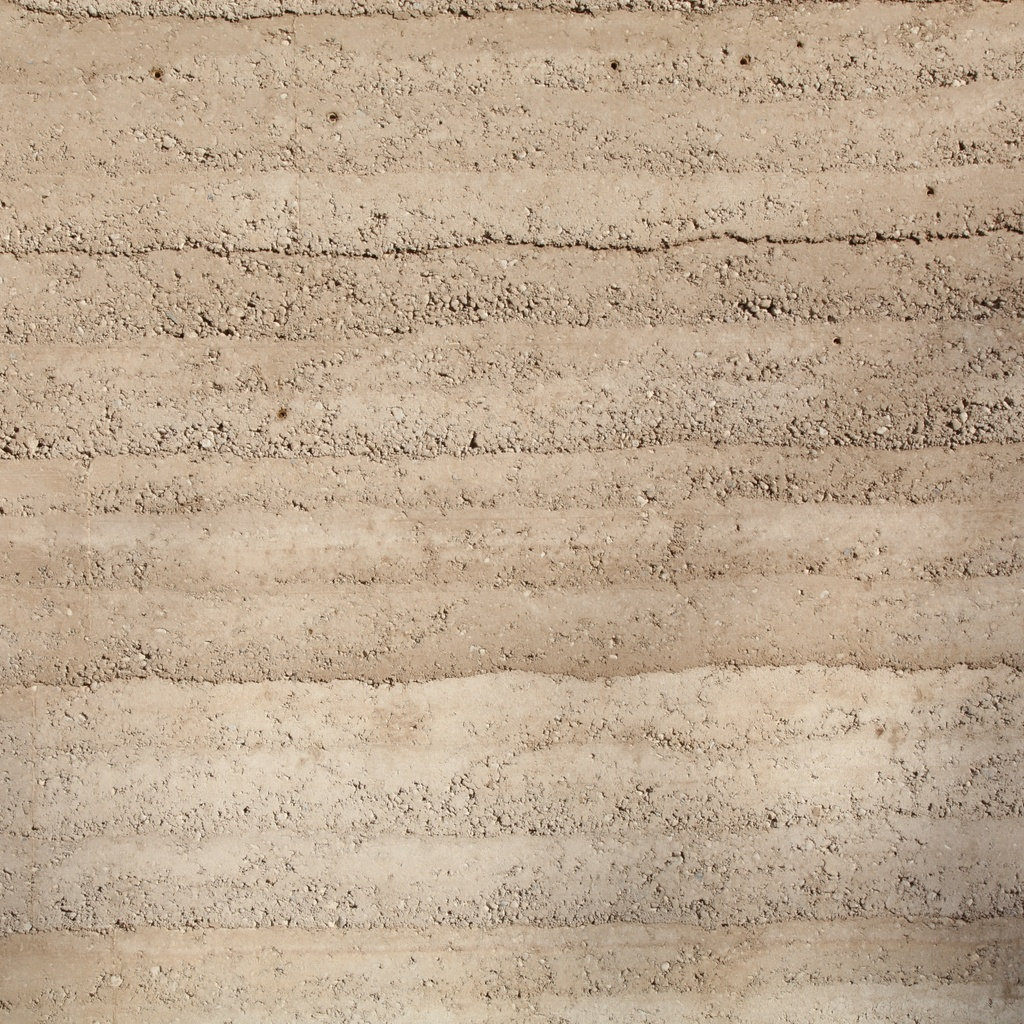
\includegraphics[width=\linewidth]{Images/LoRAs/STAMPBETON/Training_images/15.jpg} \\
    \end{tabular}
  }
  \caption{The images used to train the stampbeton LoRA.}
  \label{fig:gridstampbeton}
\end{figure}

% Upon the first training, the model seemed to be 'undertrained': in some images, there were vertical lines on the material and they were not properly captioned, so the model incorporated that into its idea of the material.\\
% \begin{figure}[H]
%     \centering
%     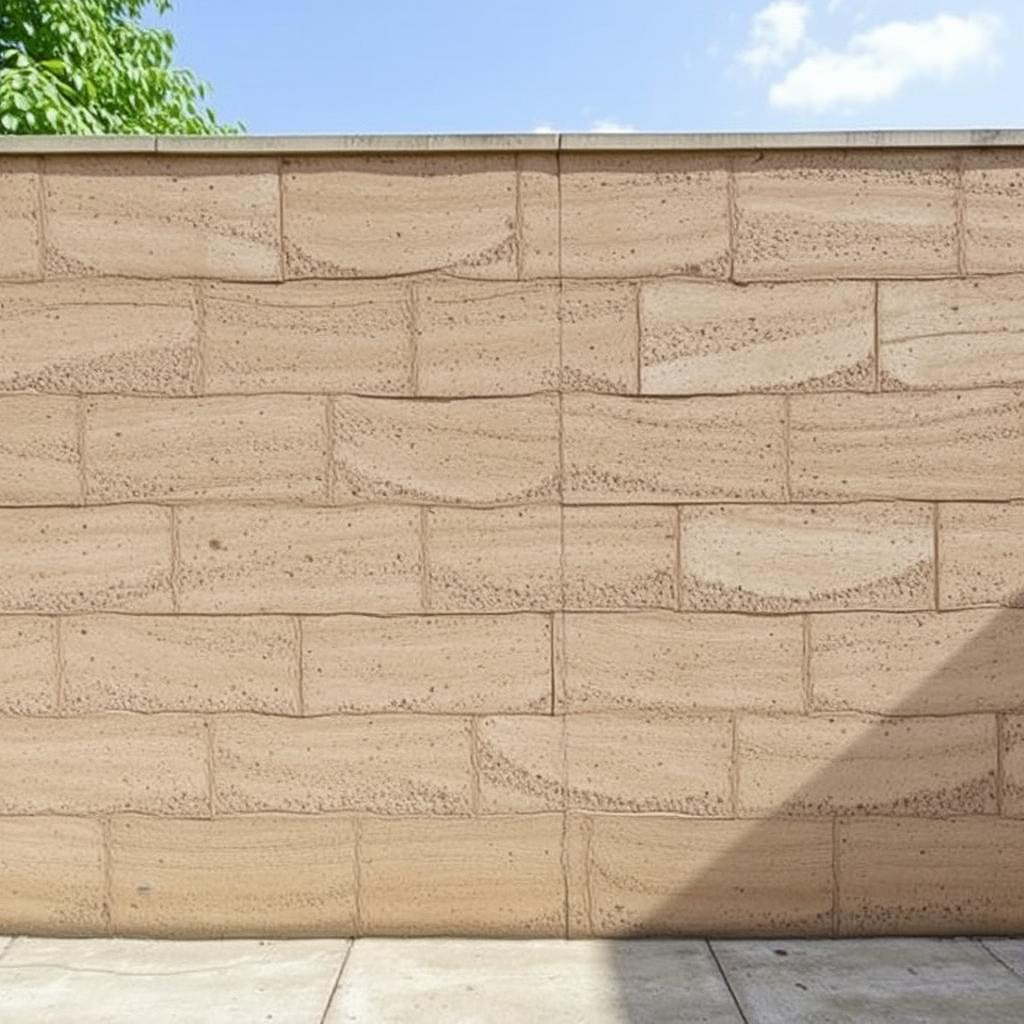
\includegraphics[width=0.5\linewidth]{afbeeldingen/STAMPBETON/v1 .png}
%     \caption{An image produced with the first stampbeton LoRA, showcasing the masonry-like texture caused by overfitting. Prompt: 'Stampbeton wall with bold horizontal strata'.}
%     \label{fig:stampbeton v1}
% \end{figure}
% For the second version, the captions were modified and this problem was, largely, resolved. The model did not give perfect images of stamped concrete 100\% of the time; sometimes, the masonry structure would pop up again, but way less than with version 1. 
% \begin{figure}[H]
%     \centering
%     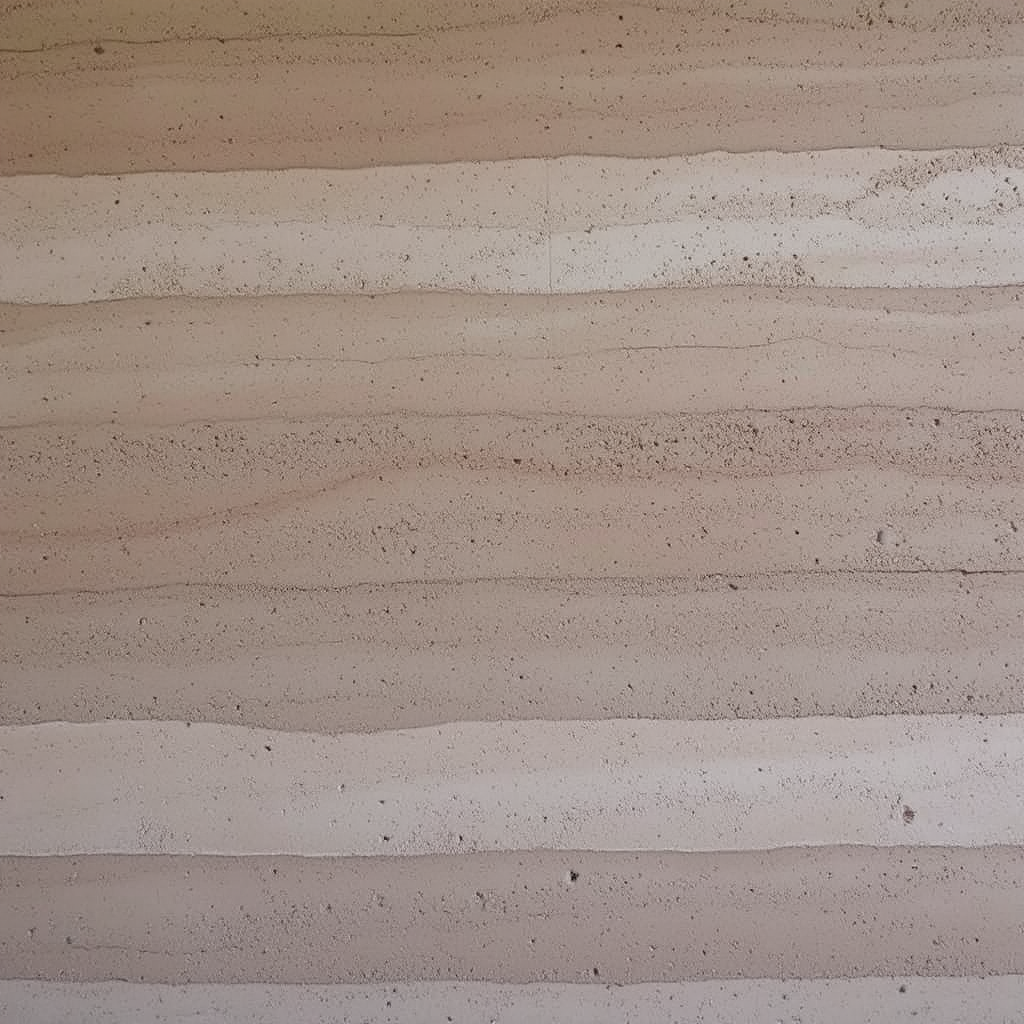
\includegraphics[width=0.5\linewidth]{afbeeldingen/STAMPBETON/v2.png}
%     \caption{An image produced with the second stampbeton LoRA, showing the structure that the model understands to be stamped concrete. Prompt: 'Stampbeton wall with bold horizontal strata'.}
%     \label{fig:stampbeton v2}
% \end{figure}

\subsubsection{3D-effect}
The second LoRA creates a 3D-effect in facades, which is obtained by adding protruding elements to the facade, such as a tent or a canopy. The purpose of creating a 3D-effect is to make the facade feel more warm inviting.\\
After validation, one image (figure \ref{fig:3deffectomittedimage}) was left out of the original dataset: the image did not suit the design-oriented preferences of the architect.
\begin{figure}[H]
    \centering
    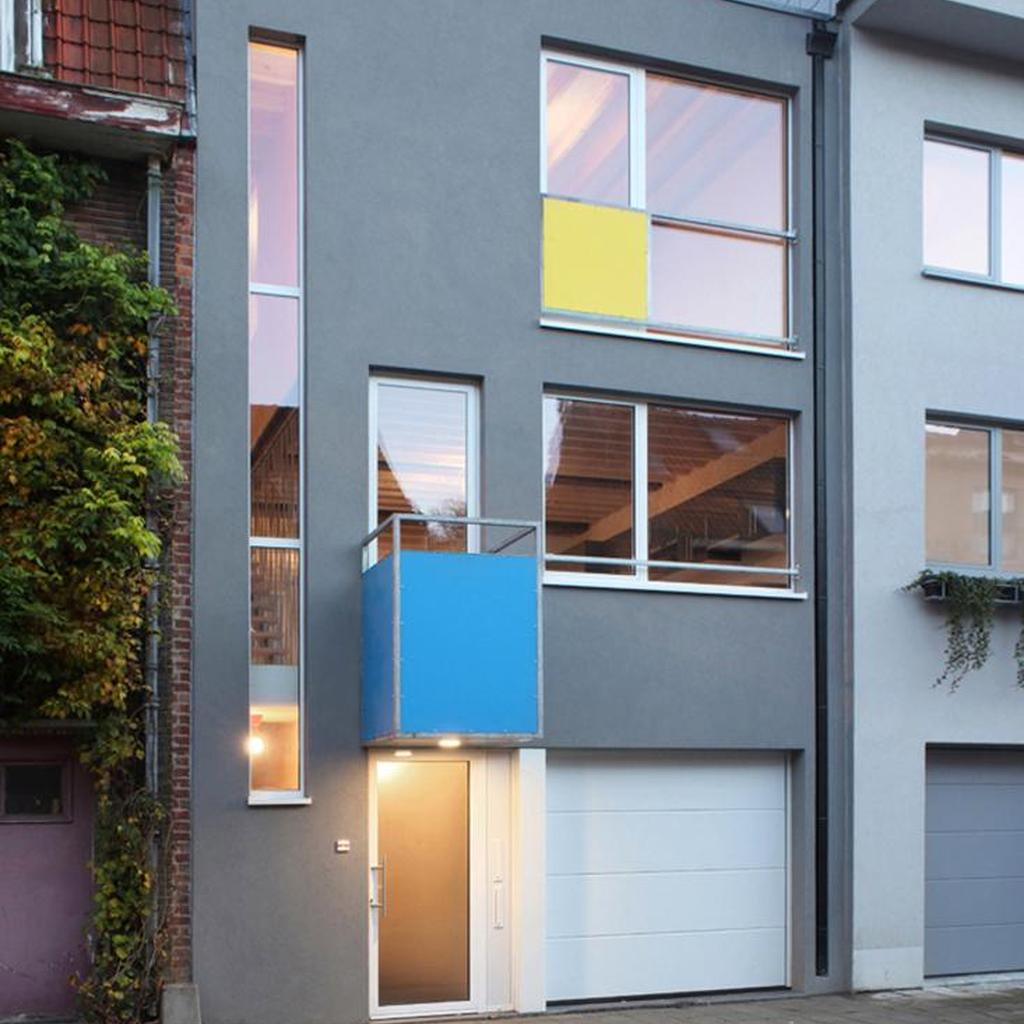
\includegraphics[width=0.24\linewidth]{Images//LoRAs//3D-effect/4.jpg}
    \caption{The image removed from the original 3D-effect dataset.}
    \label{fig:3deffectomittedimage}
\end{figure}
Figure \ref{fig:grid3D-effect} portrays the training images for this LoRA.
\begin{figure}[H]
  \centering
  \resizebox{\textwidth}{!}{%
    \begin{tabular}{@{}ccccc@{}}
      % Row 1: images 1–5
      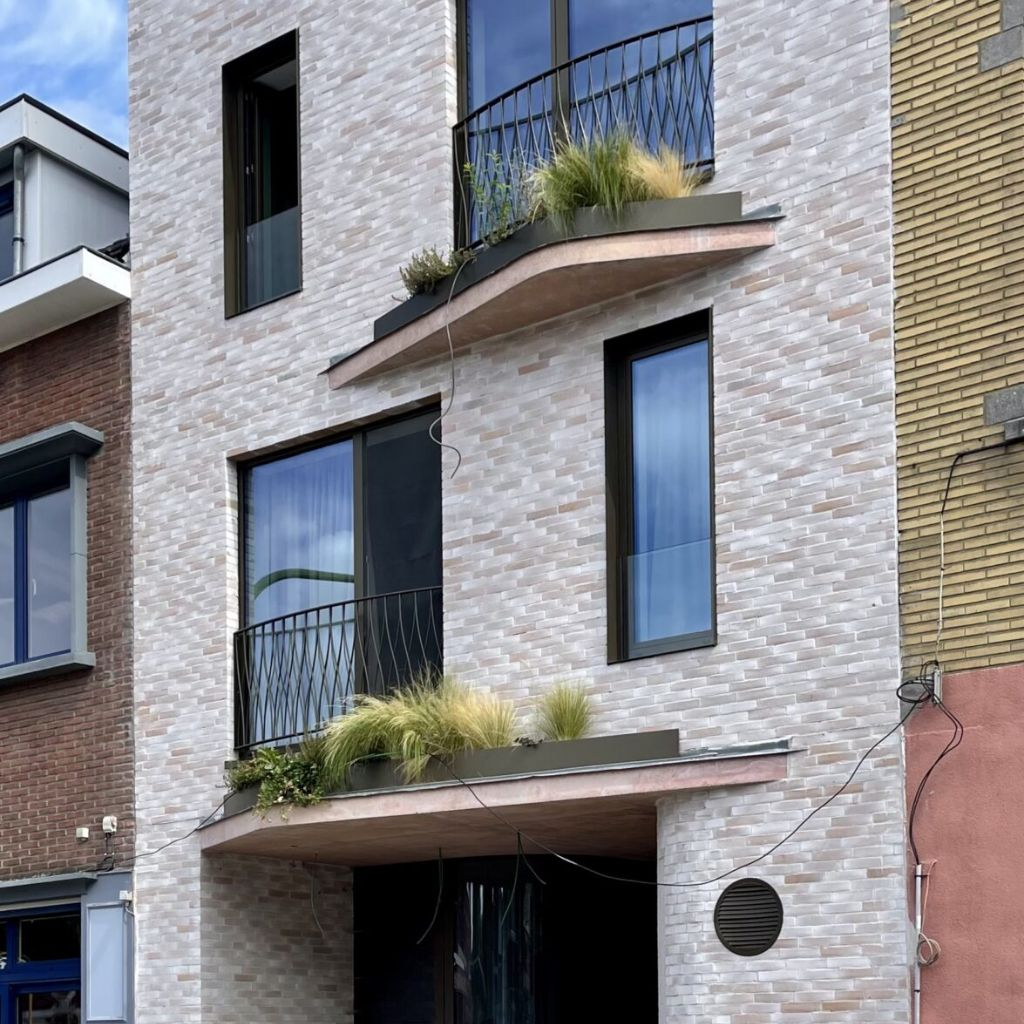
\includegraphics[width=\linewidth]{Images/LoRAs/3D-effect/Training_images/1.jpeg} &
      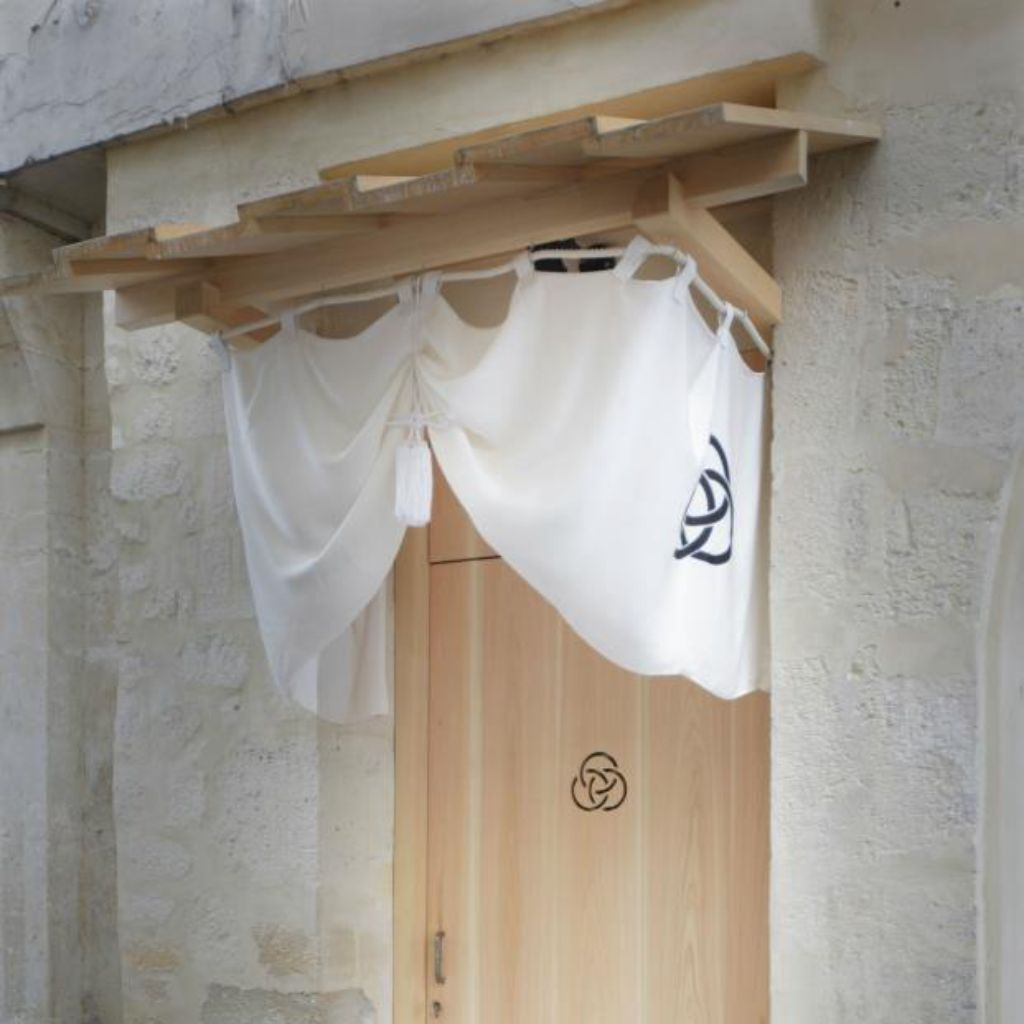
\includegraphics[width=\linewidth]{Images/LoRAs/3D-effect/Training_images/2.jpg} &
      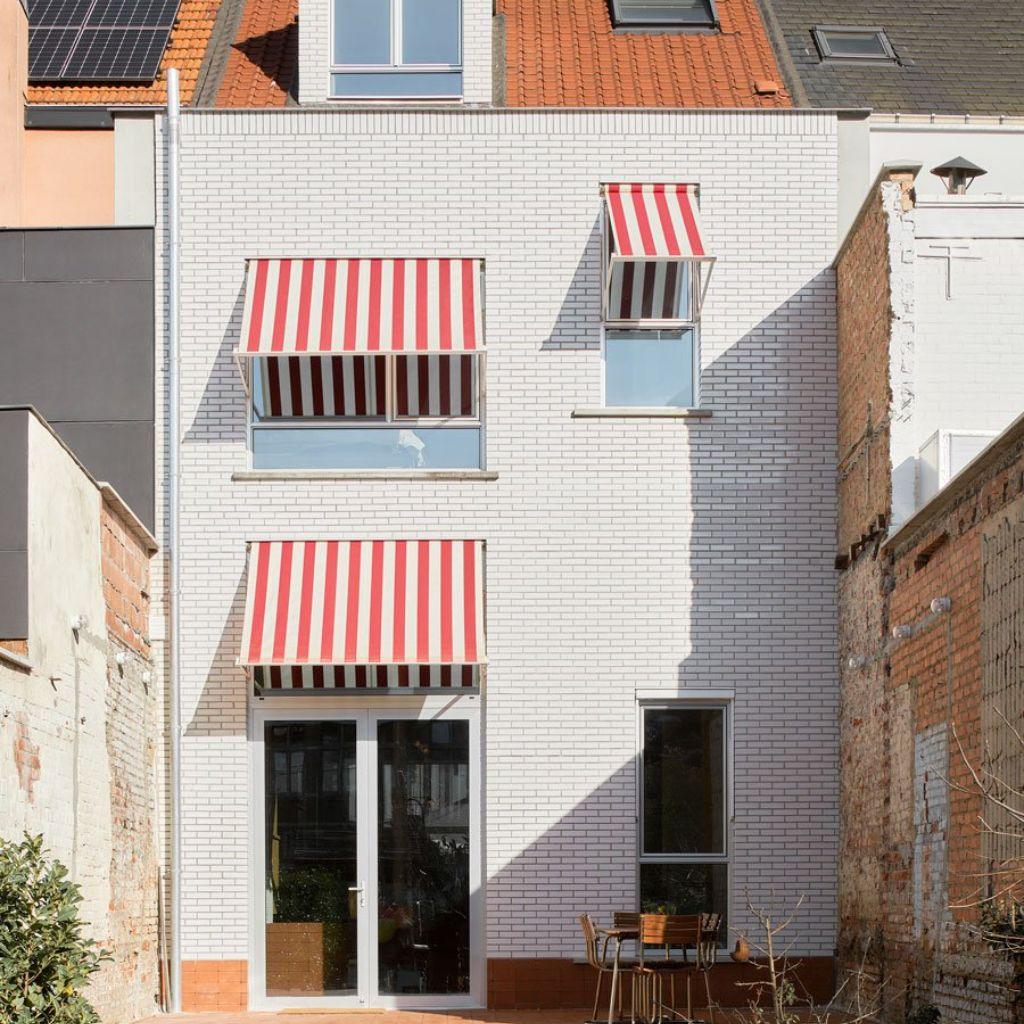
\includegraphics[width=\linewidth]{Images/LoRAs/3D-effect/Training_images/3.jpg} &
      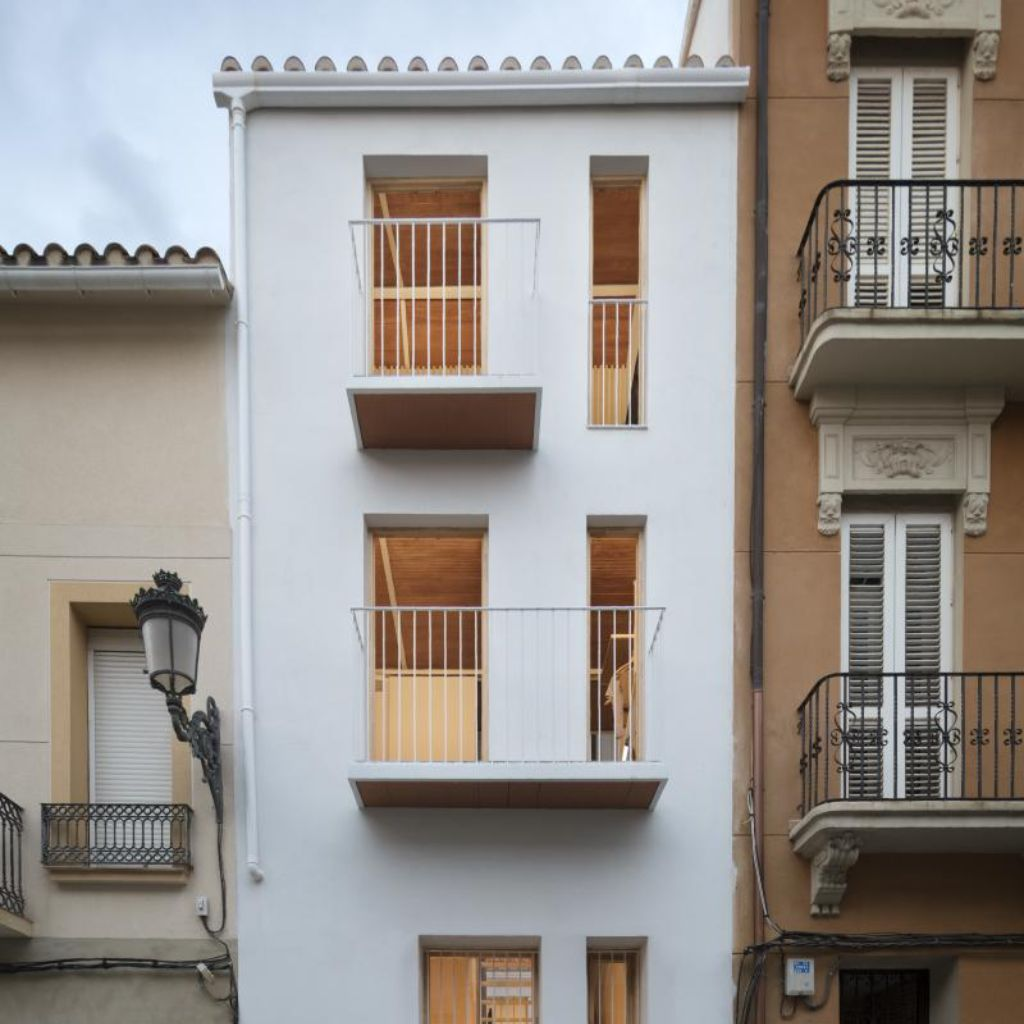
\includegraphics[width=\linewidth]{Images/LoRAs/3D-effect/Training_images/4.jpg} &
      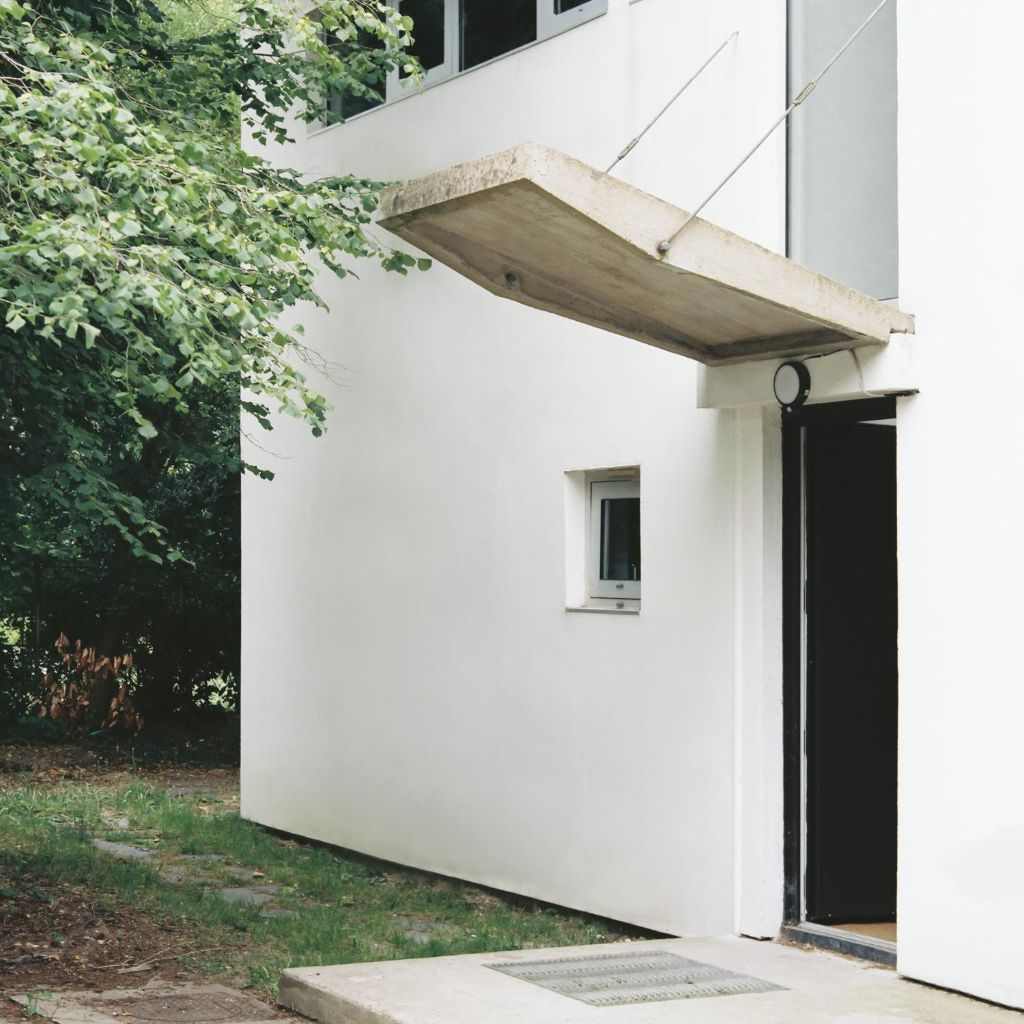
\includegraphics[width=\linewidth]{Images/LoRAs/3D-effect/Training_images/5.jpg} \\[2pt]

      % Row 2: images 6–10
      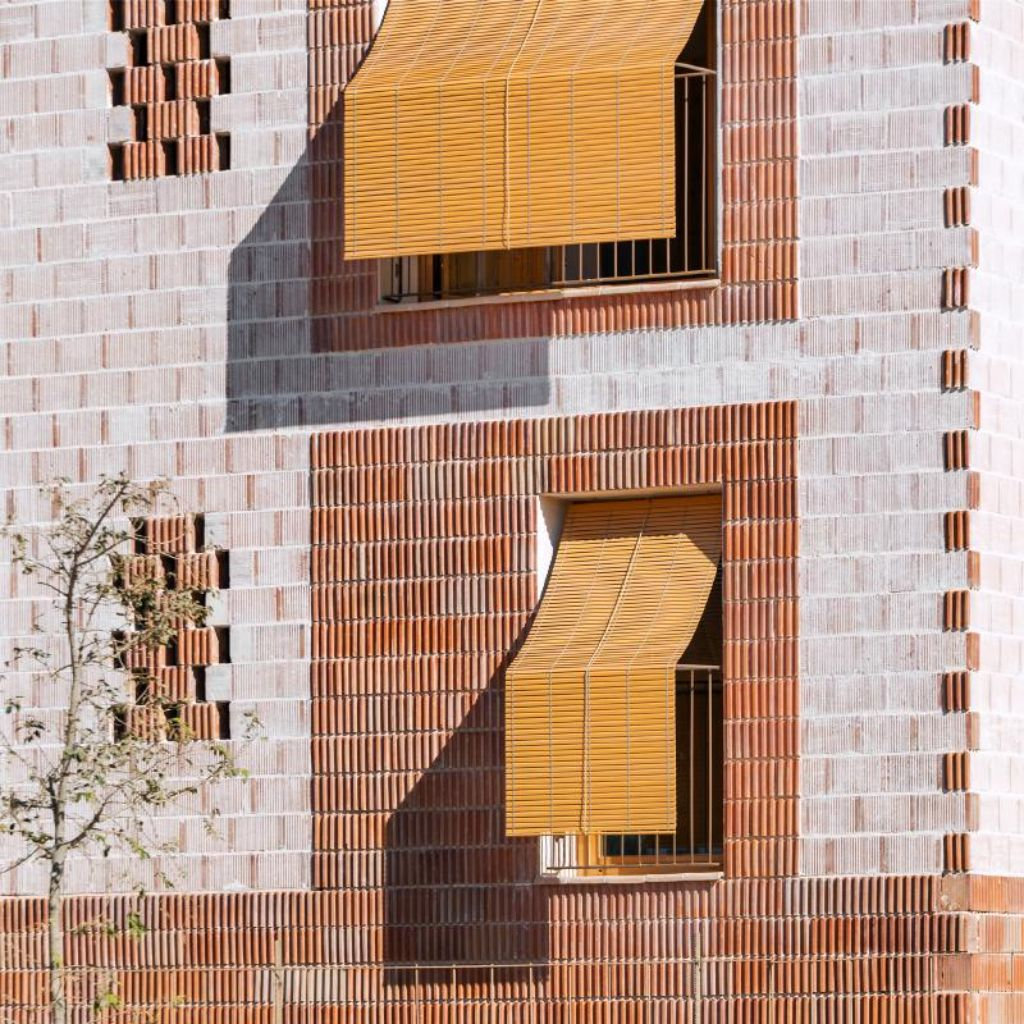
\includegraphics[width=\linewidth]{Images/LoRAs/3D-effect/Training_images/6.jpg} &
      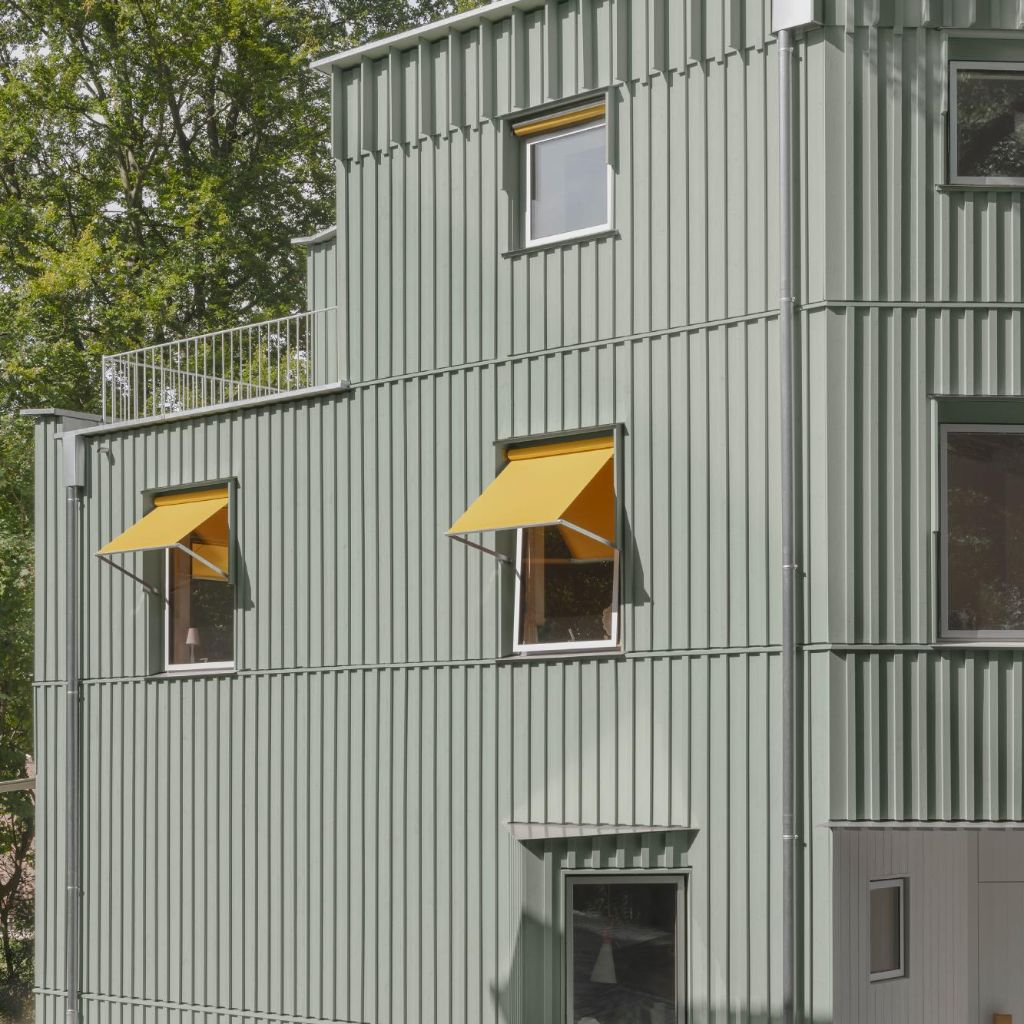
\includegraphics[width=\linewidth]{Images/LoRAs/3D-effect/Training_images/7.jpg} &
      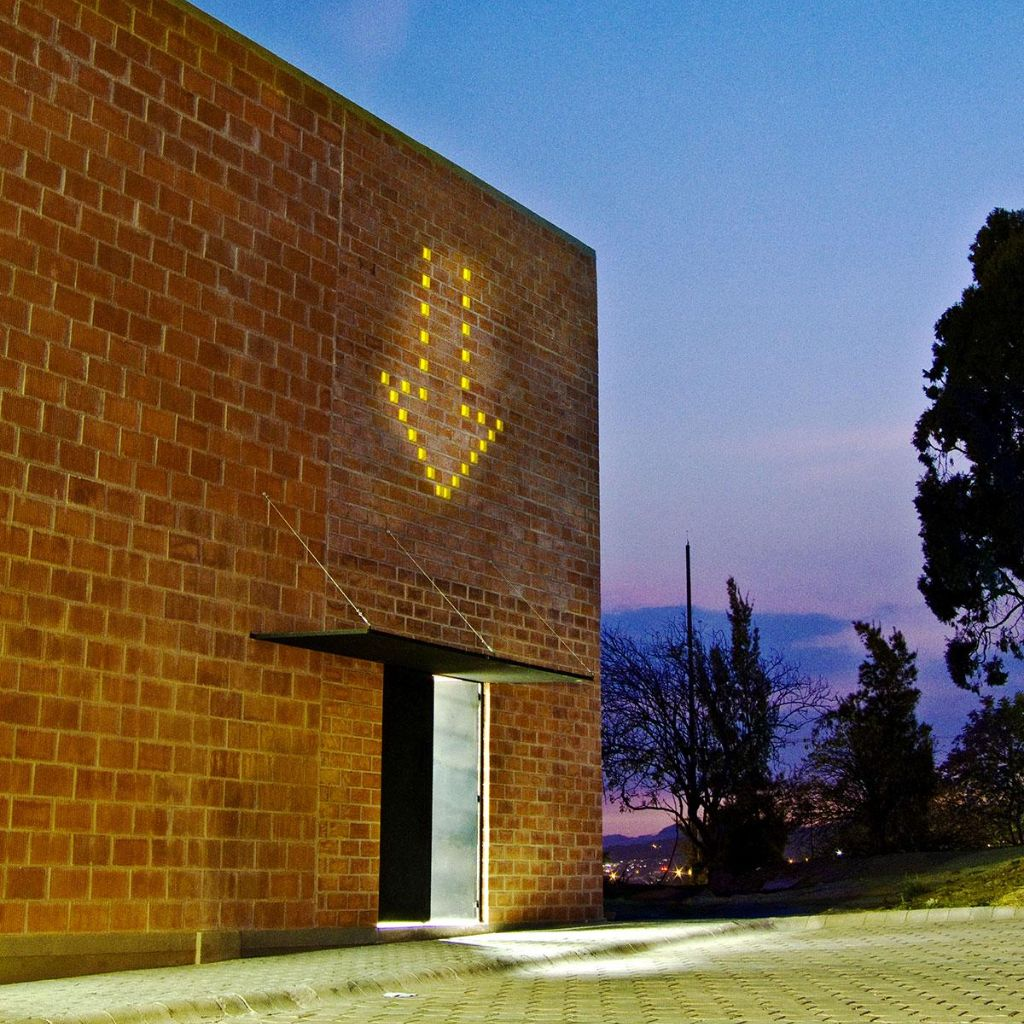
\includegraphics[width=\linewidth]{Images/LoRAs/3D-effect/Training_images/8.jpg} &
      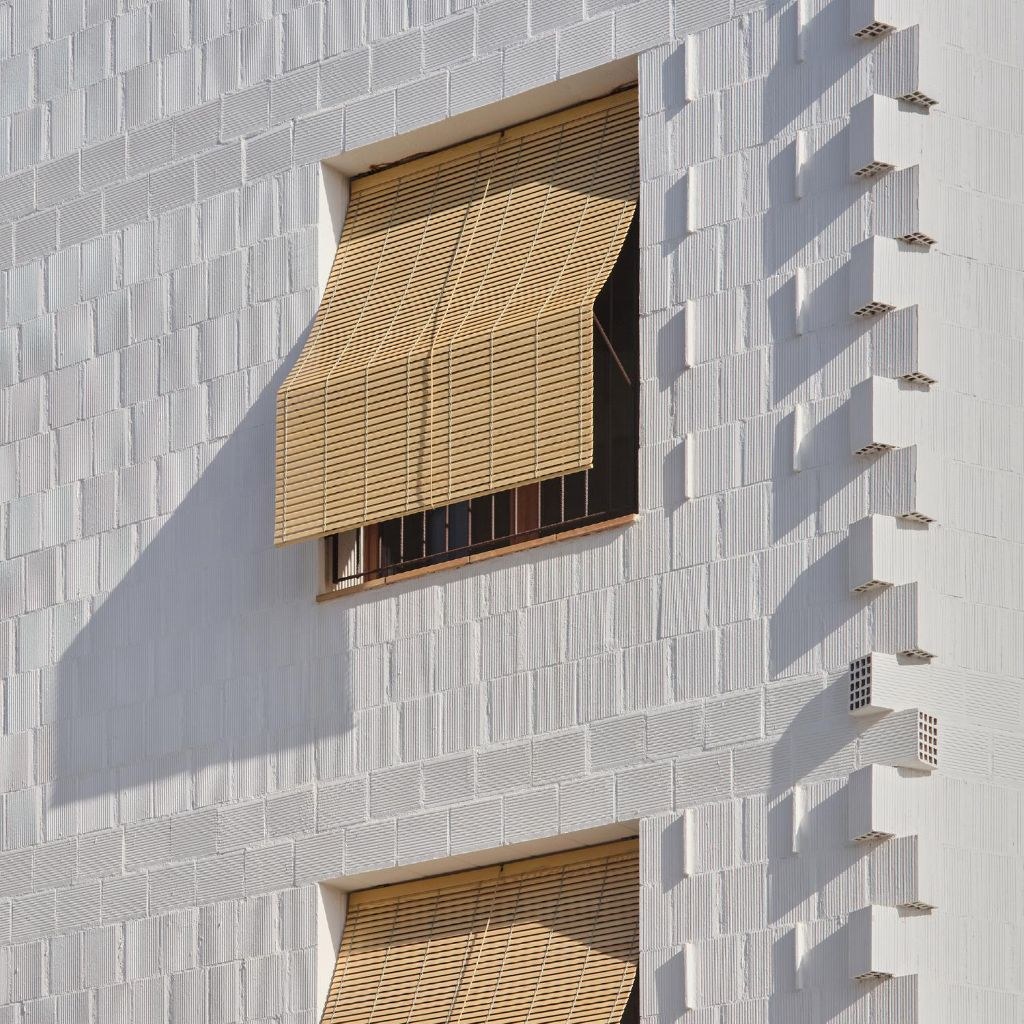
\includegraphics[width=\linewidth]{Images/LoRAs/3D-effect/Training_images/9.jpg} &
      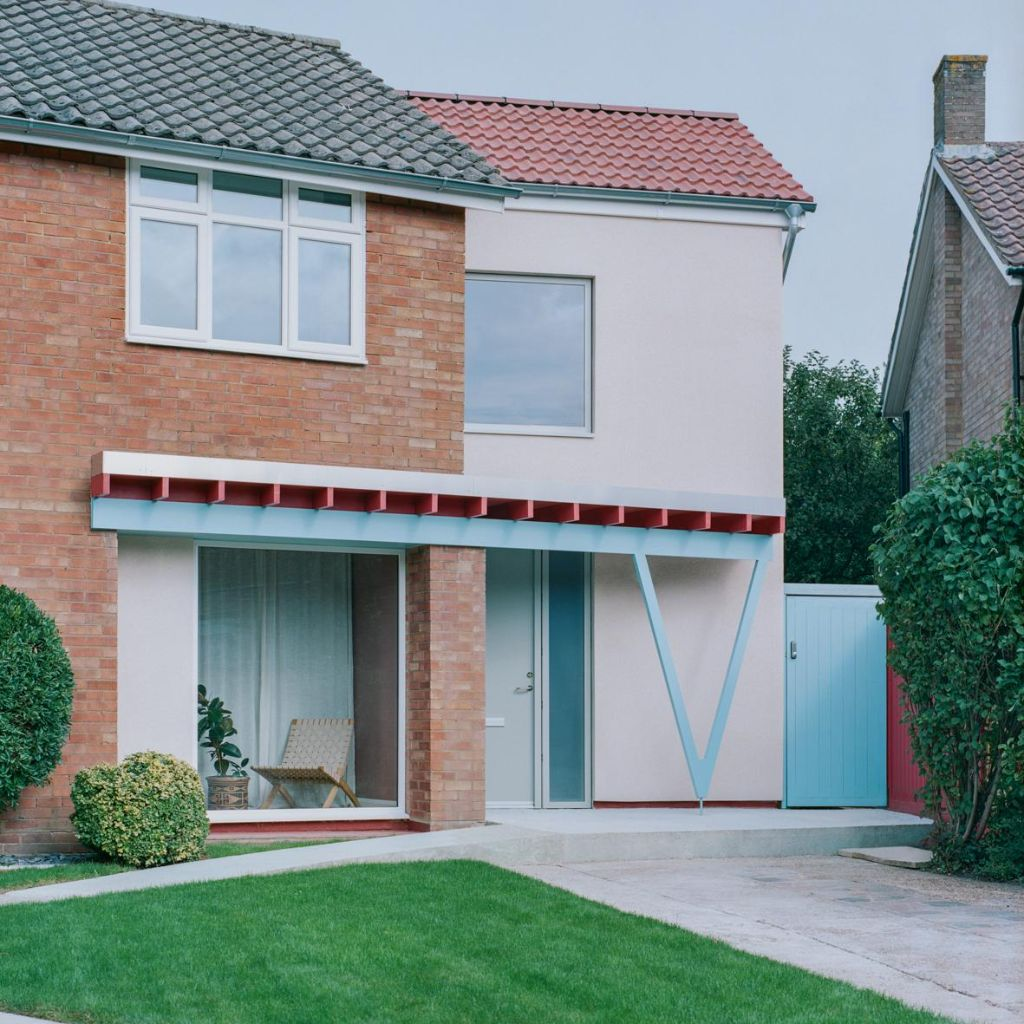
\includegraphics[width=\linewidth]{Images/LoRAs/3D-effect/Training_images/10.jpg} \\[2pt]

      % Row 3: images 11–15
      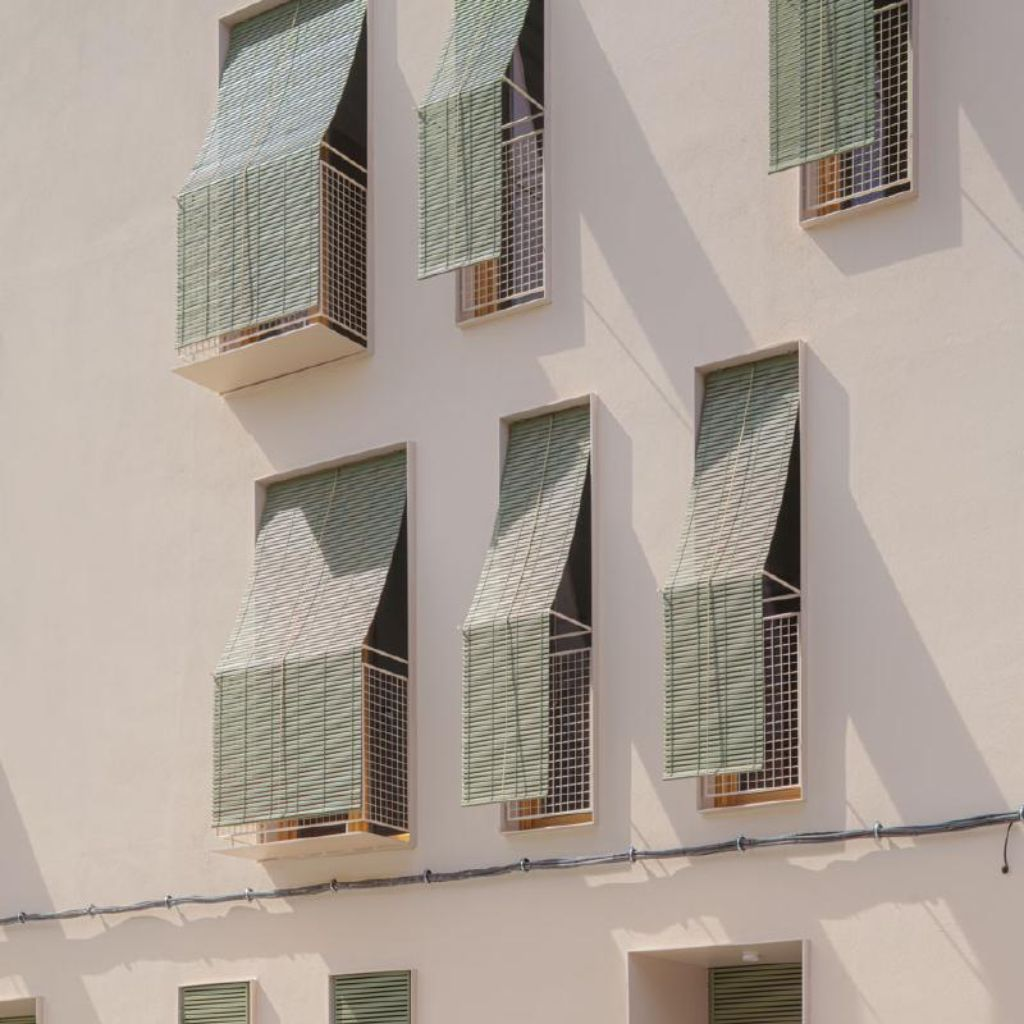
\includegraphics[width=\linewidth]{Images/LoRAs/3D-effect/Training_images/11.jpg} &
      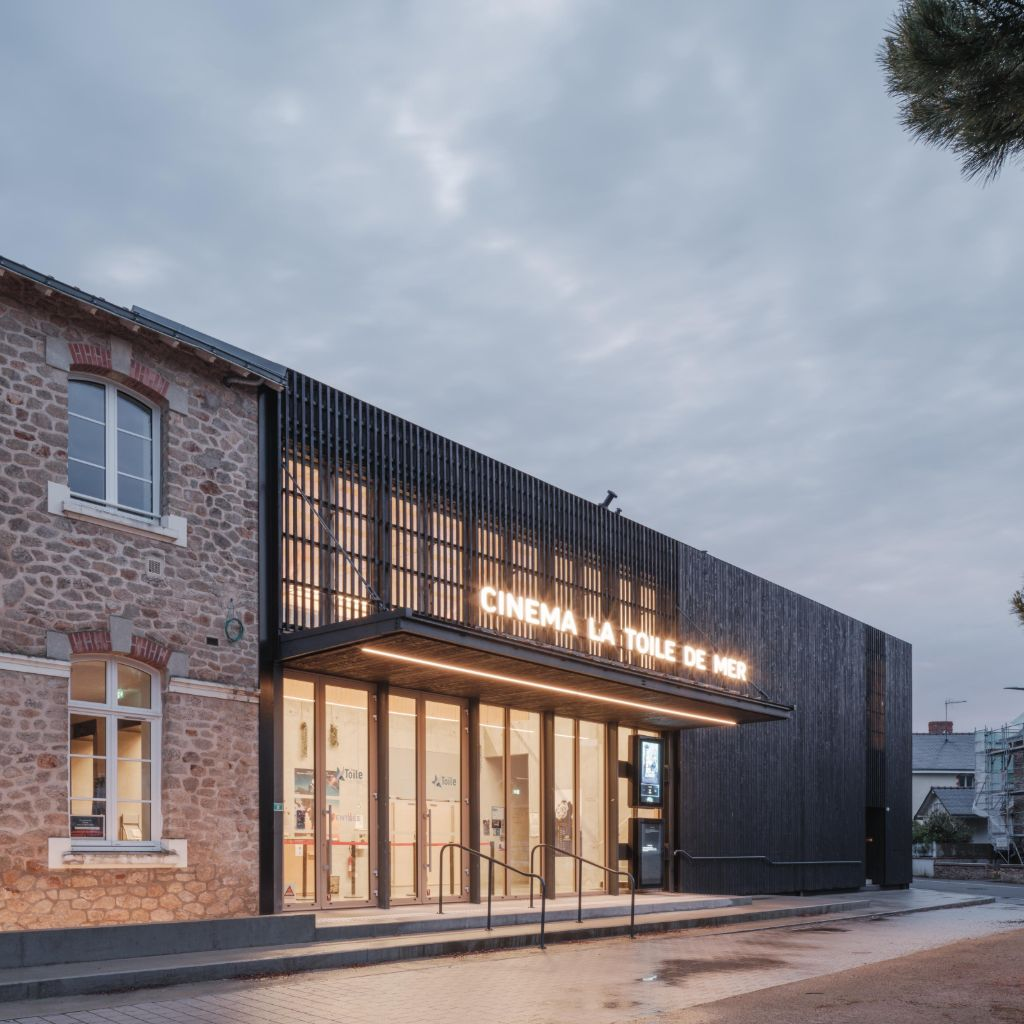
\includegraphics[width=\linewidth]{Images/LoRAs/3D-effect/Training_images/12.jpg} &
      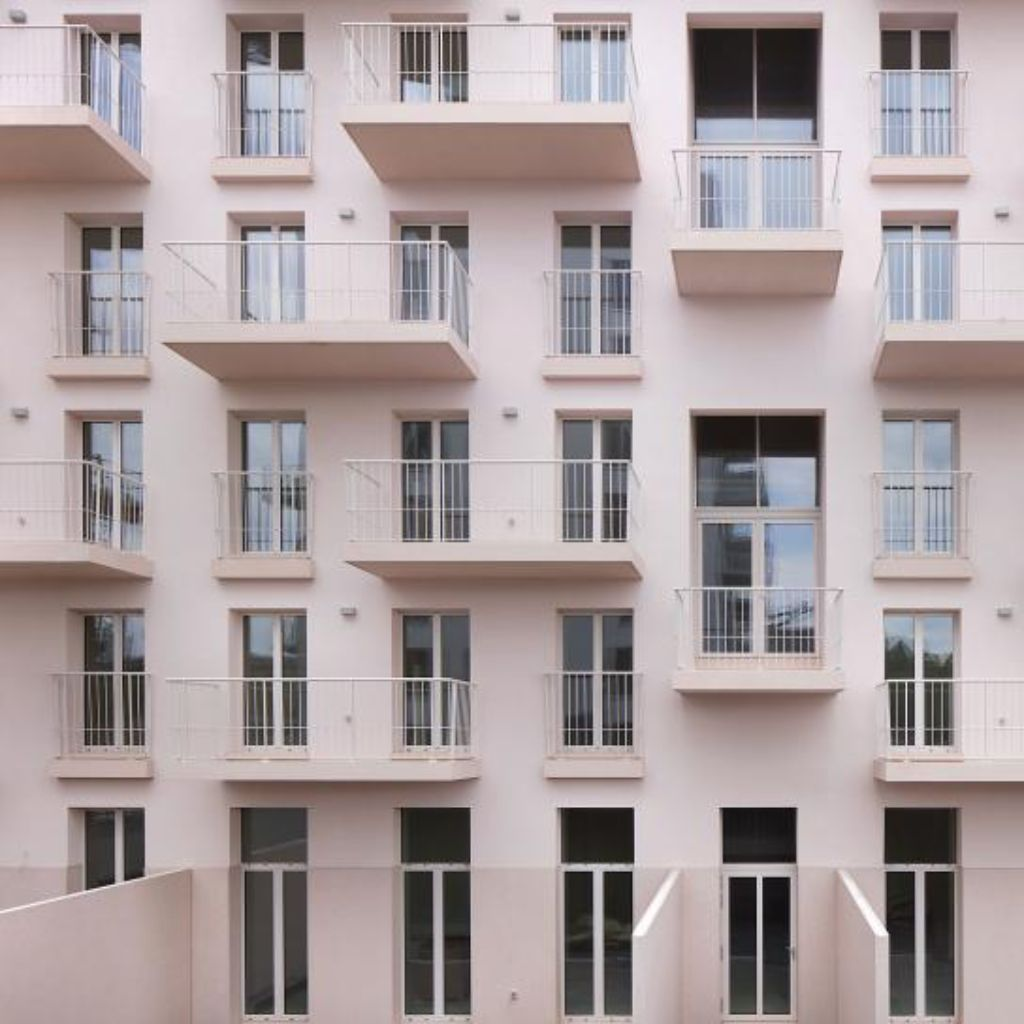
\includegraphics[width=\linewidth]{Images/LoRAs/3D-effect/Training_images/13.jpg} &
      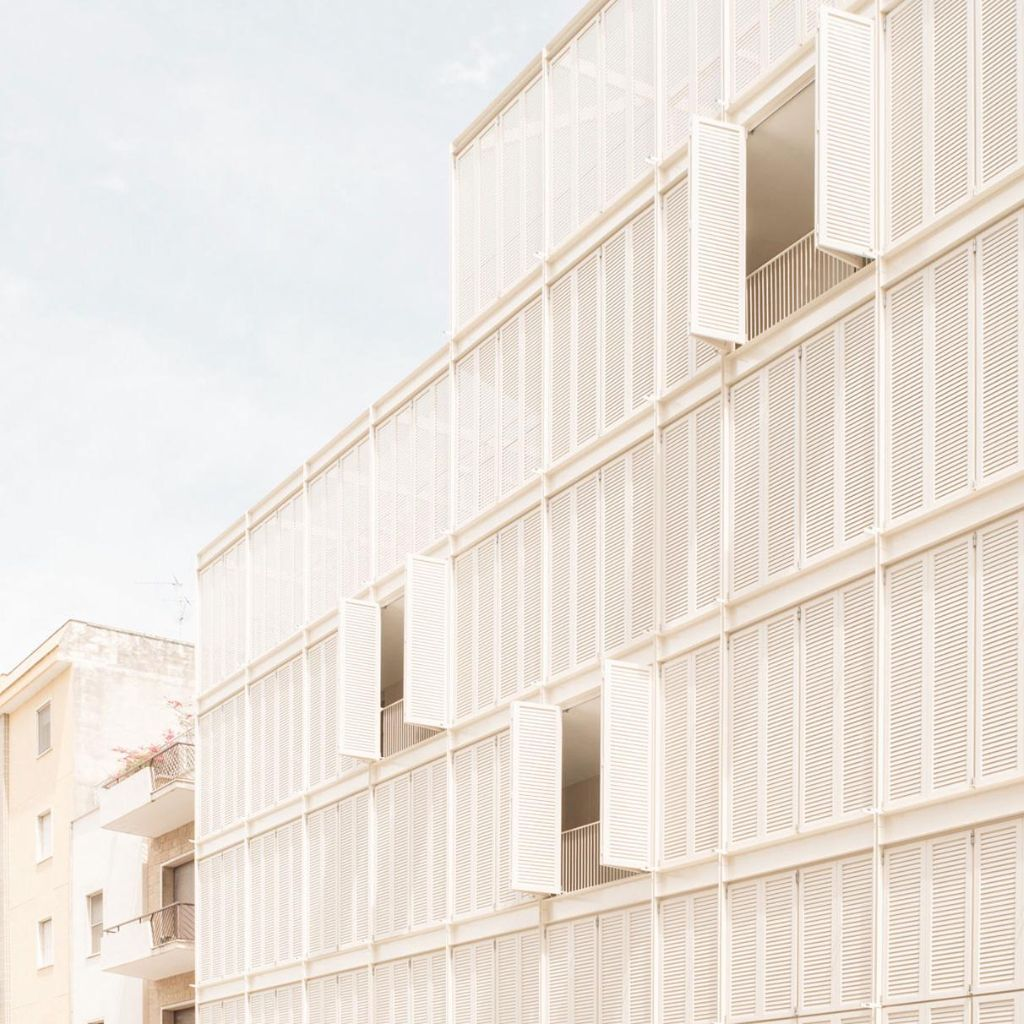
\includegraphics[width=\linewidth]{Images/LoRAs/3D-effect/Training_images/14.jpg} &
      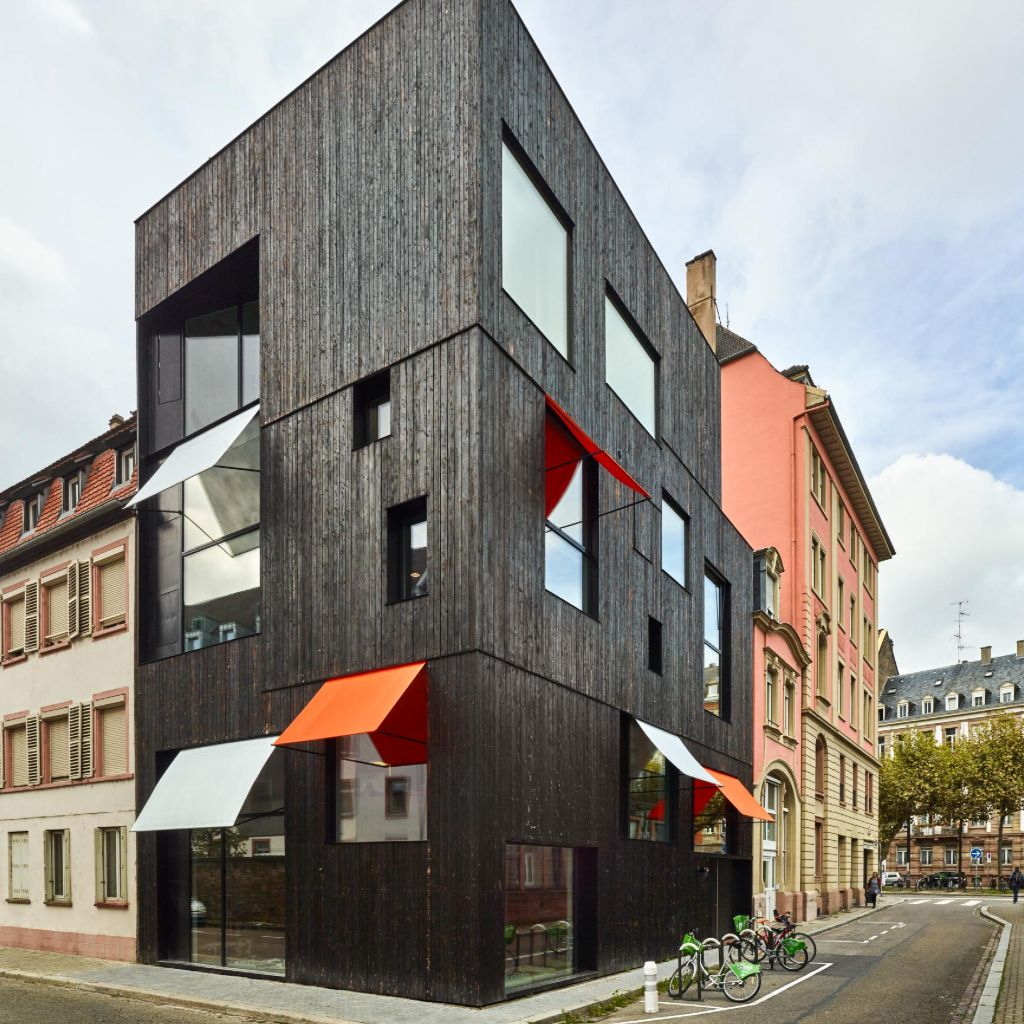
\includegraphics[width=\linewidth]{Images/LoRAs/3D-effect/Training_images/15.jpg} \\
    \end{tabular}%
  }
  \caption{The images used to train the 3D-effect LoRA.}
  \label{fig:grid3D-effect}
\end{figure}

\subsubsection{Geleding}
The third and last LoRA for DMOA replicates the concept of dividing two floors from each other in the facade. The architect expressed that he likes to do this to divide large facades into parts that are more on the human scale.\\
After validation, 5 images were left out of the original dataset. The reasons were because of too much varying depth (images 1, 2 and 4), design considerations (image 3) and the division being limited to the wooden 'skin' (image 5).
\begin{figure}[H]
  \centering
  \resizebox{\textwidth}{!}{%
    \begin{tabular}{@{}ccccc@{}}
      % Row 1: images 1–5
      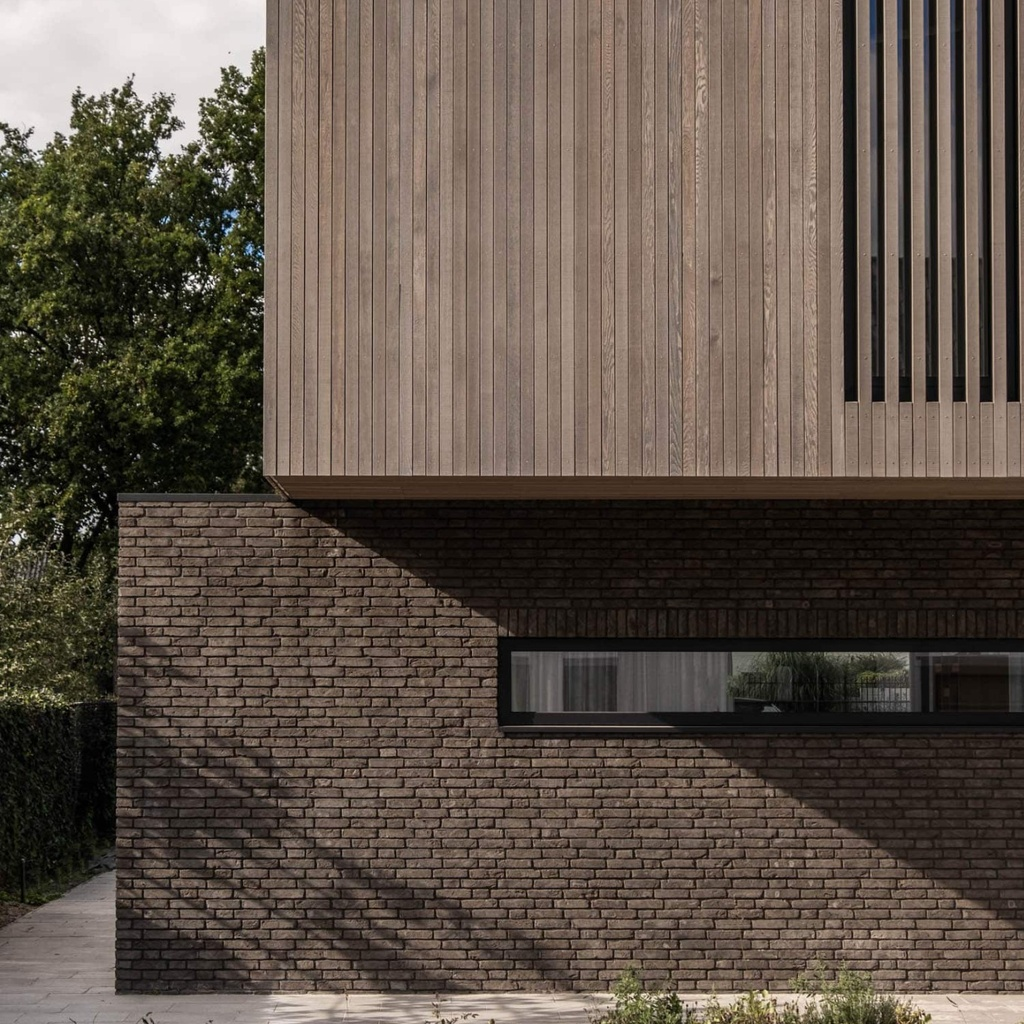
\includegraphics[width=\linewidth]{Images/LoRAs/Geleding/8.jpg} &
      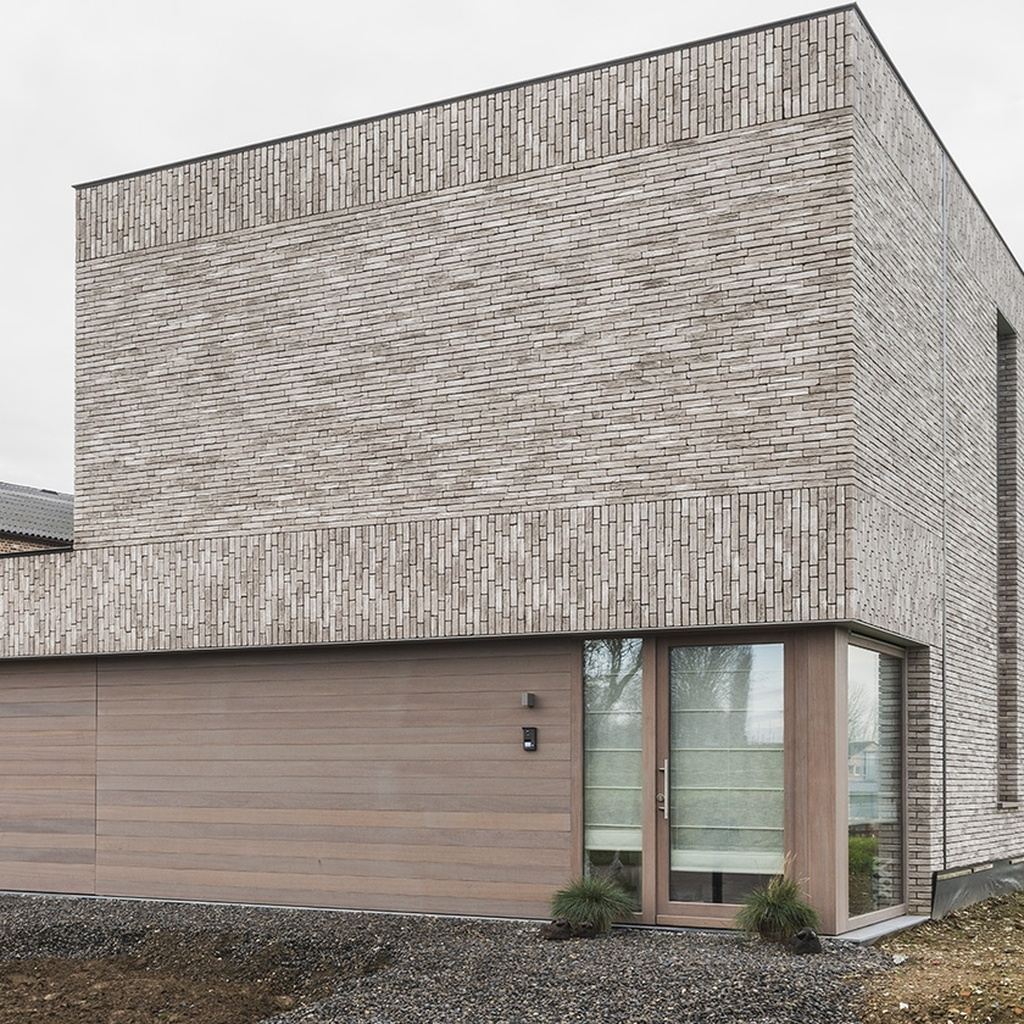
\includegraphics[width=\linewidth]{Images/LoRAs/Geleding/9.jpg} &
      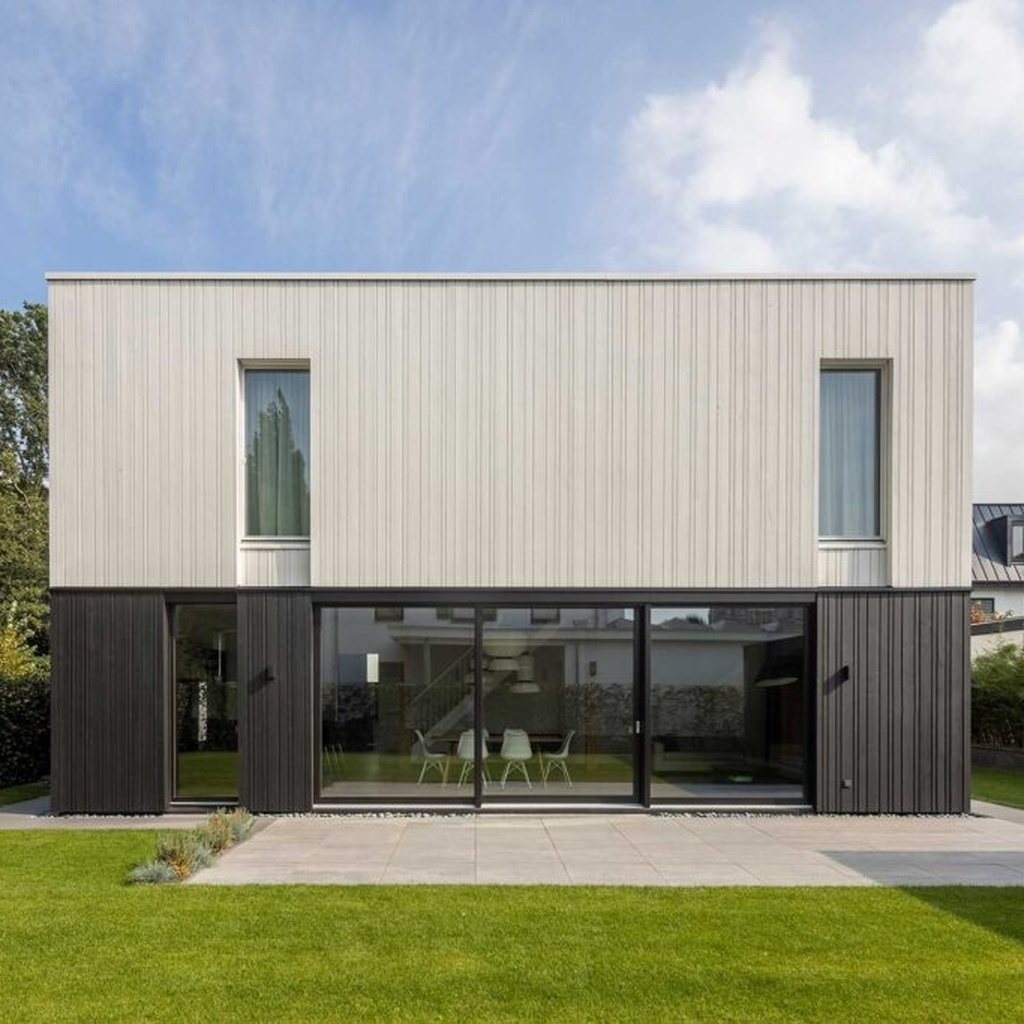
\includegraphics[width=\linewidth]{Images/LoRAs/Geleding/11.jpg} &
      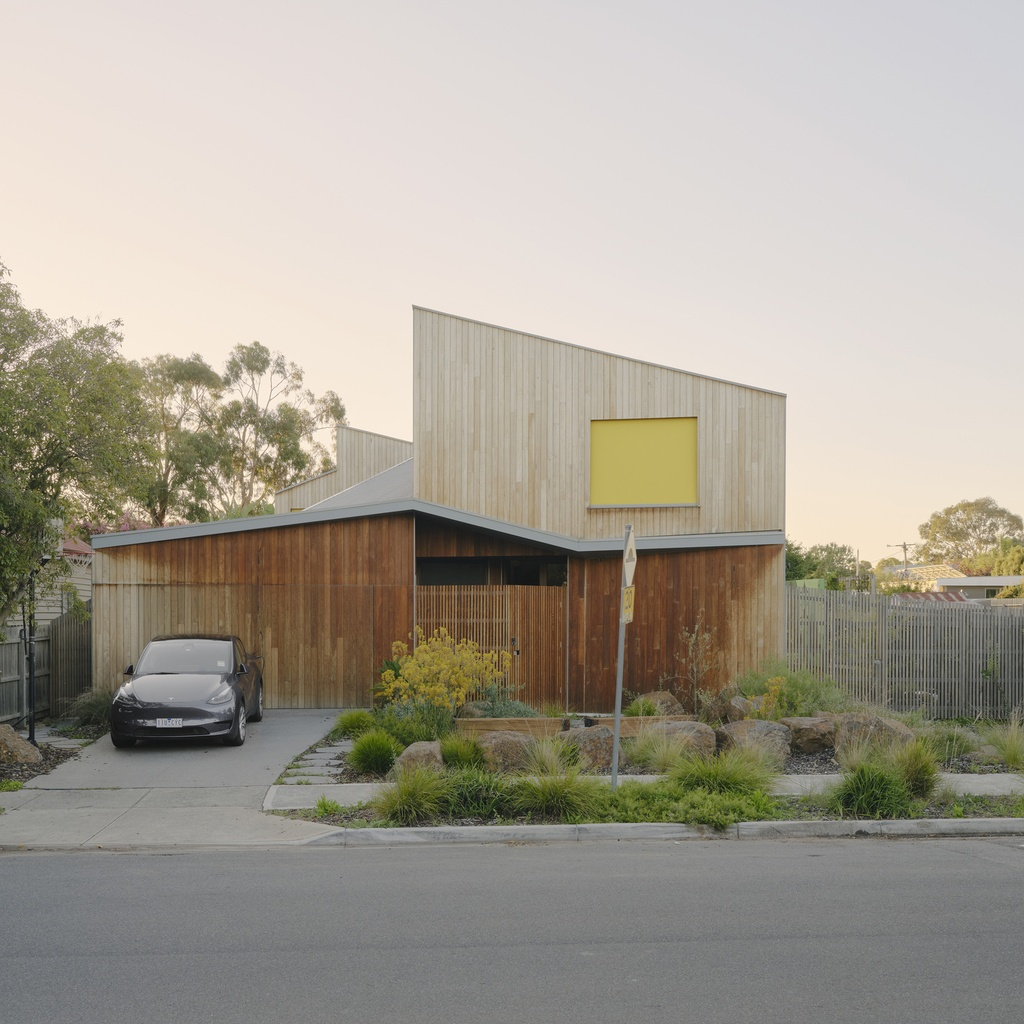
\includegraphics[width=\linewidth]{Images/LoRAs/Geleding/12.jpg} &
      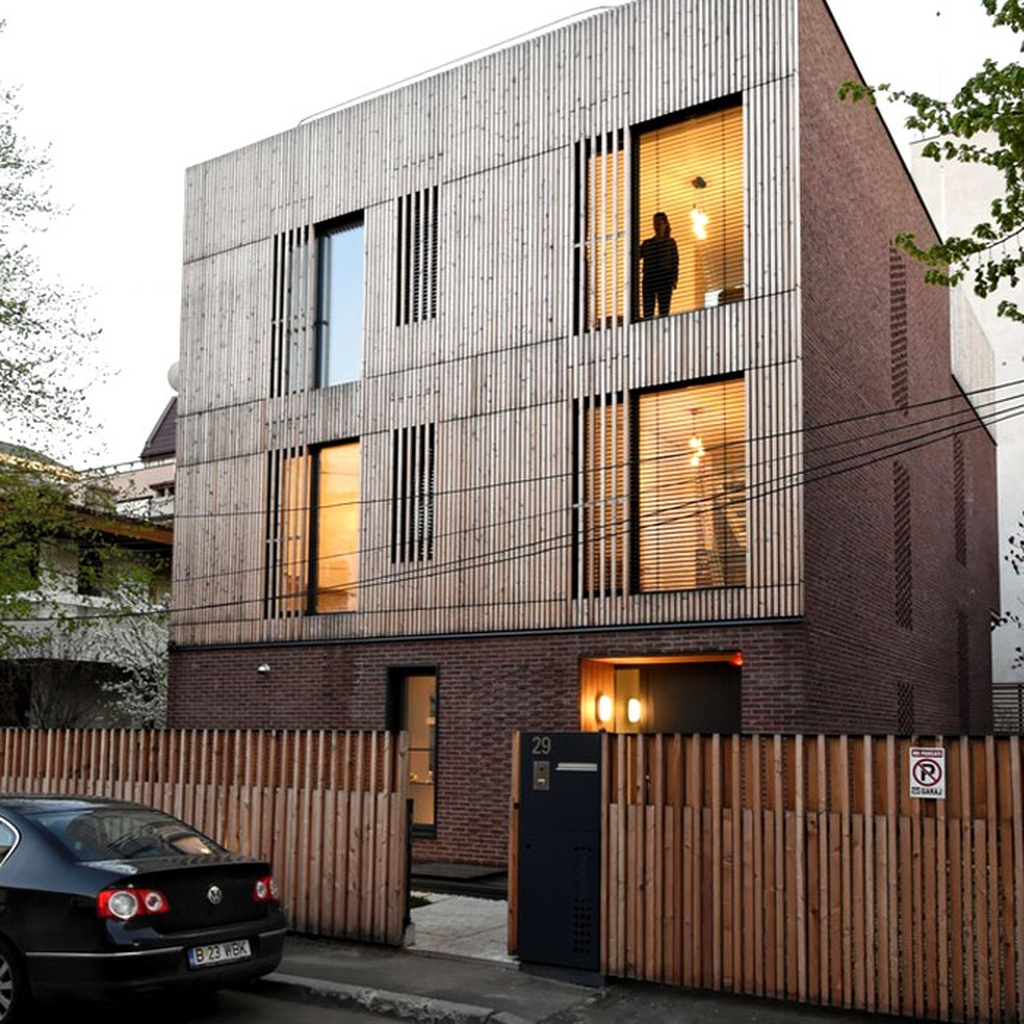
\includegraphics[width=\linewidth]{Images/LoRAs/Geleding/16.jpg} \\[2pt]
    \end{tabular}
    }
  \caption{The images removed from the original geleding dataset.}
  \label{fig:removedgeleding}
\end{figure}
Figure \ref{fig:gridgeleding} portrays the training images for this LoRA.
\begin{figure}[H]
  \centering
  \resizebox{\textwidth}{!}{%
    \begin{tabular}{@{}ccccc@{}}
      % Row 1: images 1–5
      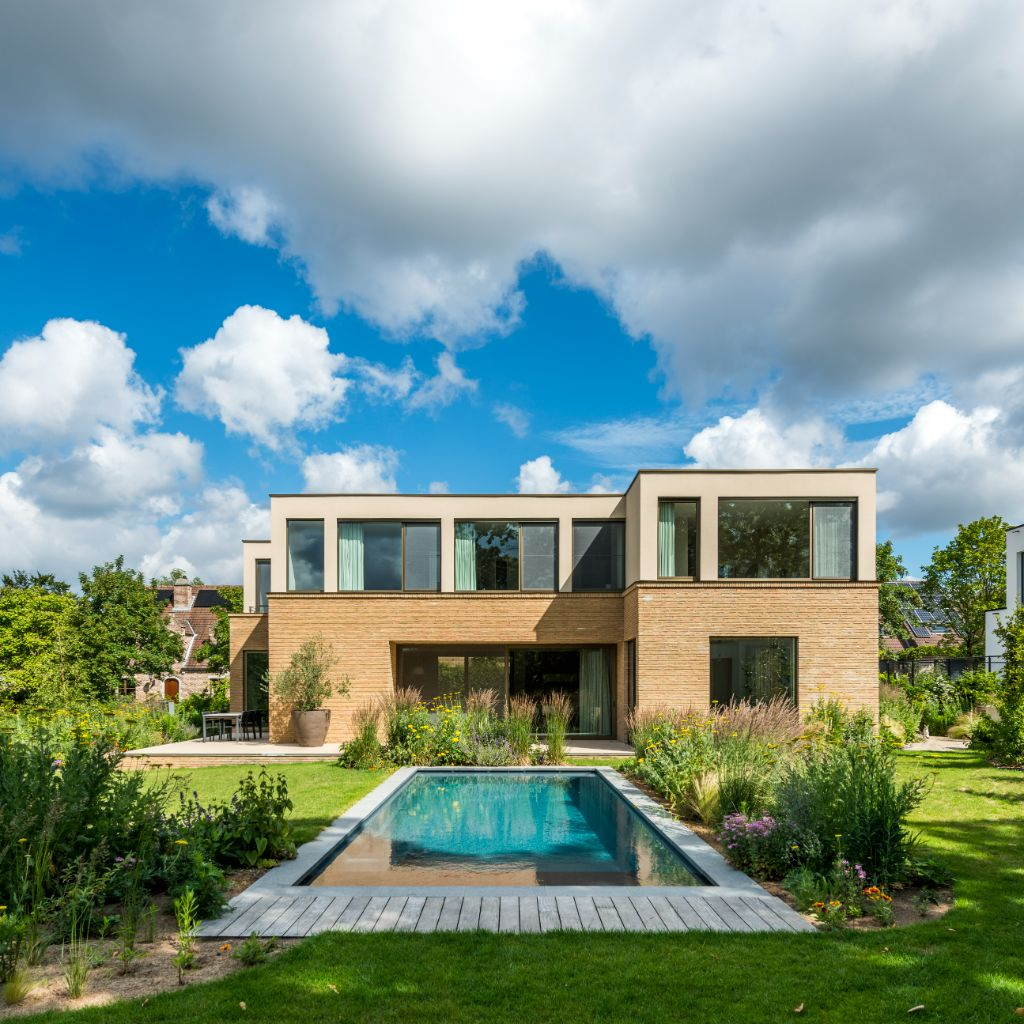
\includegraphics[width=\linewidth]{Images/LoRAs/Geleding/Training_images/1.jpg} &
      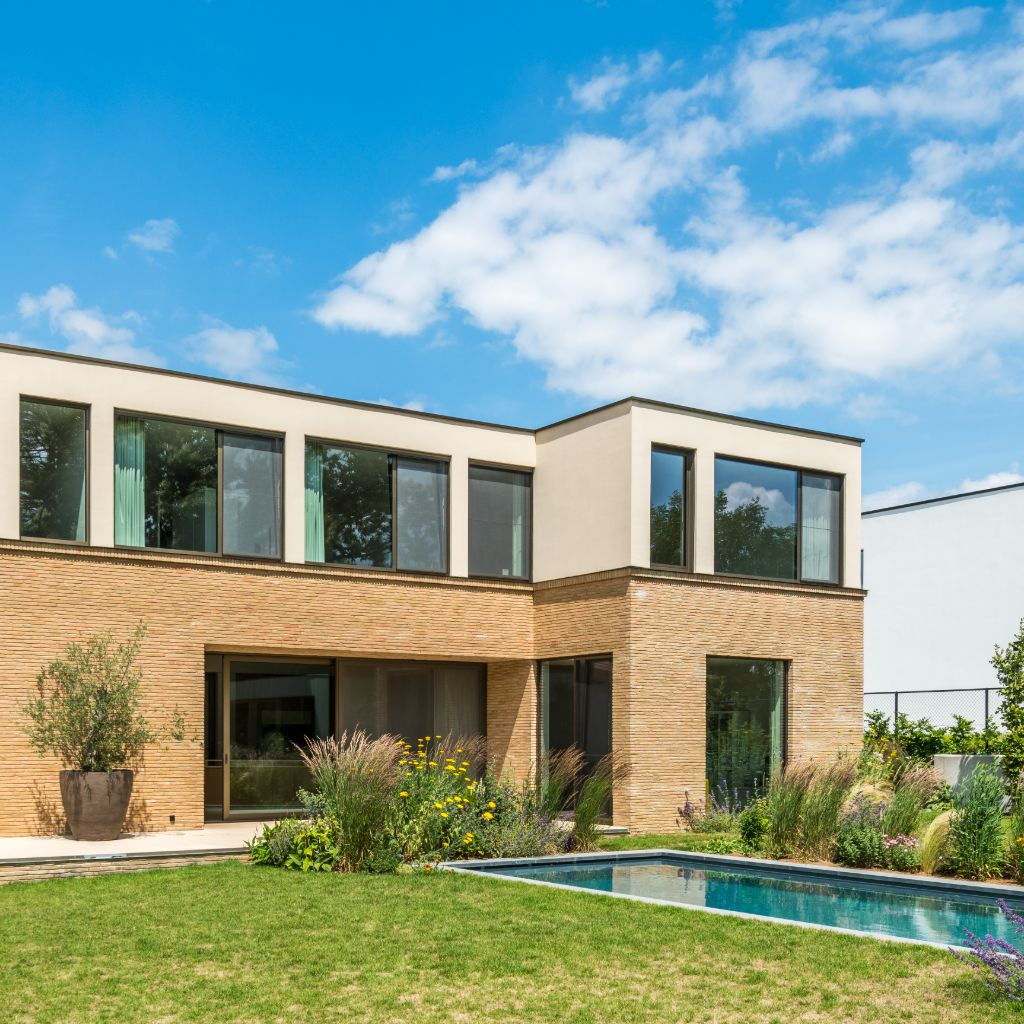
\includegraphics[width=\linewidth]{Images/LoRAs/Geleding/Training_images/2.jpg} &
      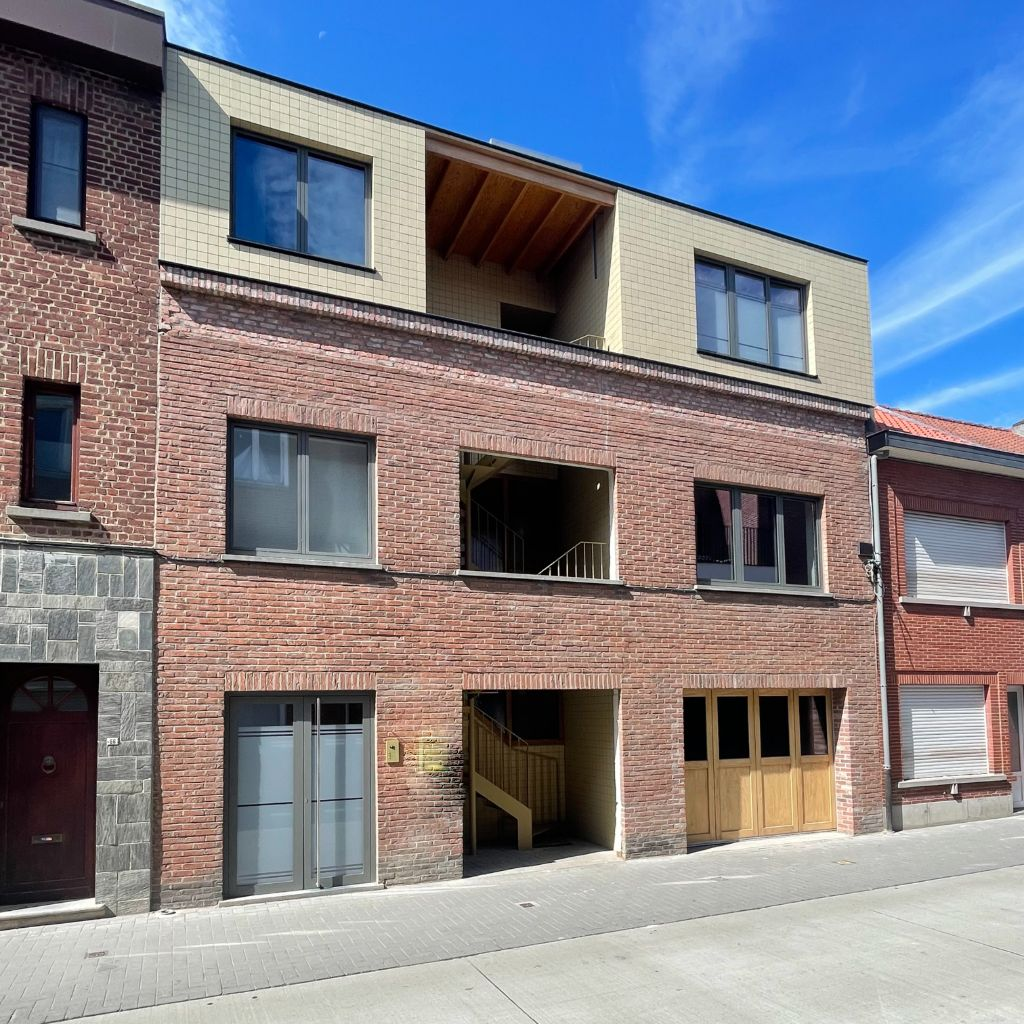
\includegraphics[width=\linewidth]{Images/LoRAs/Geleding/Training_images/3.jpeg} &
      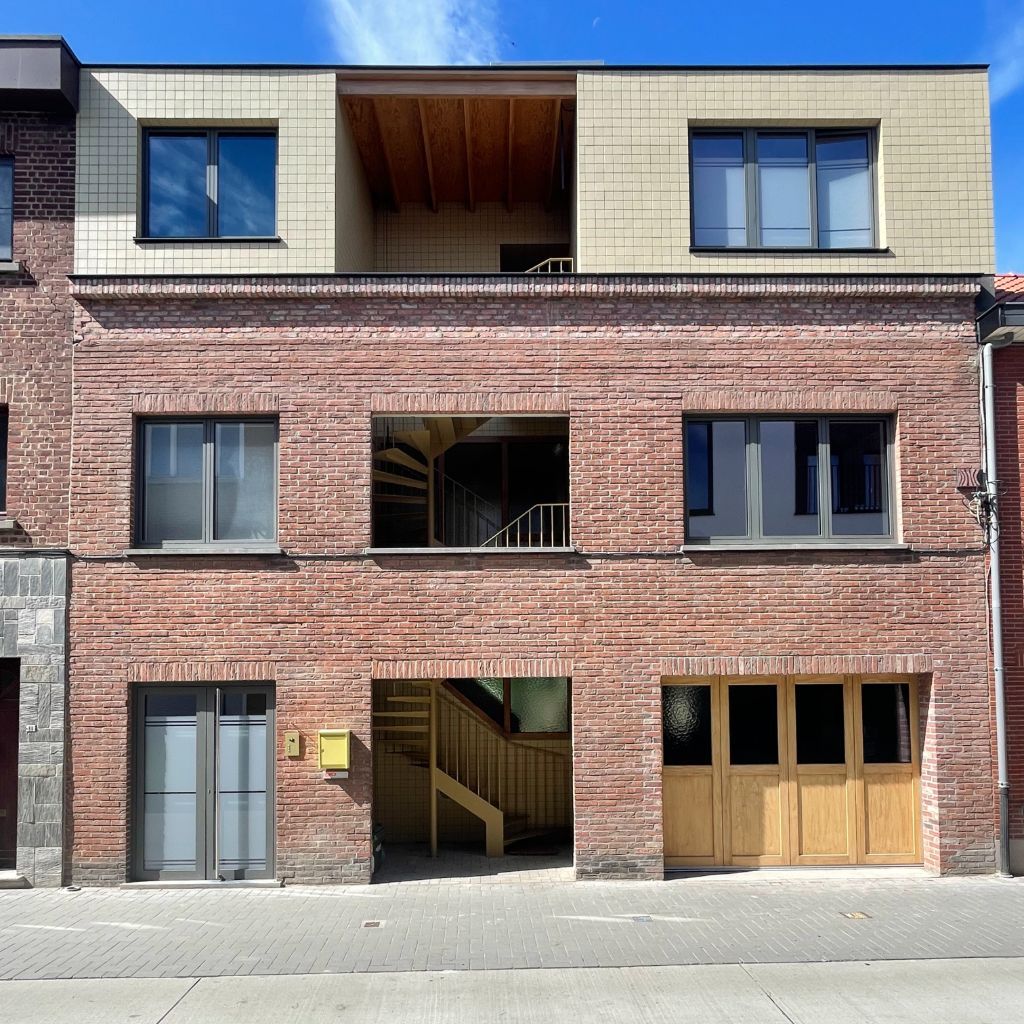
\includegraphics[width=\linewidth]{Images/LoRAs/Geleding/Training_images/4.jpeg} &
      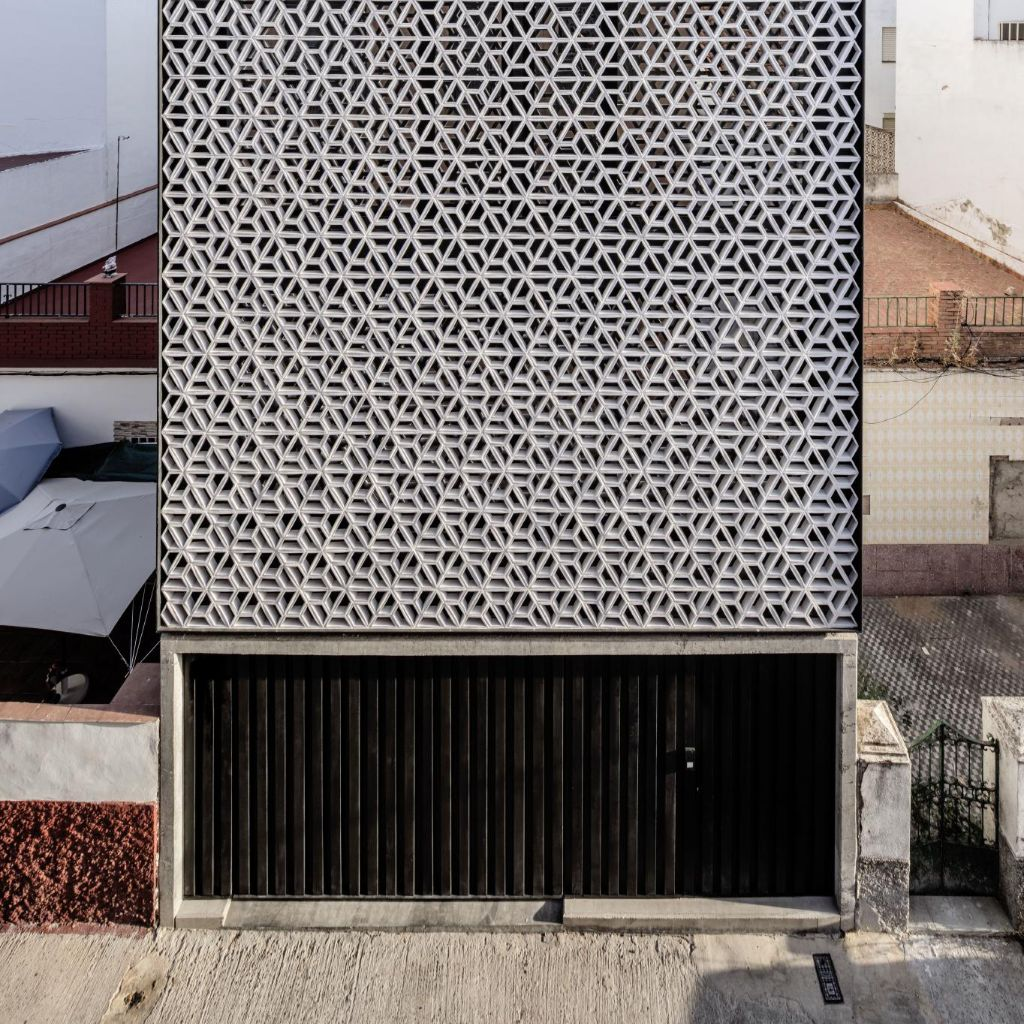
\includegraphics[width=\linewidth]{Images/LoRAs/Geleding/Training_images/5.jpg} \\[2pt]

      % Row 2: images 6–10
      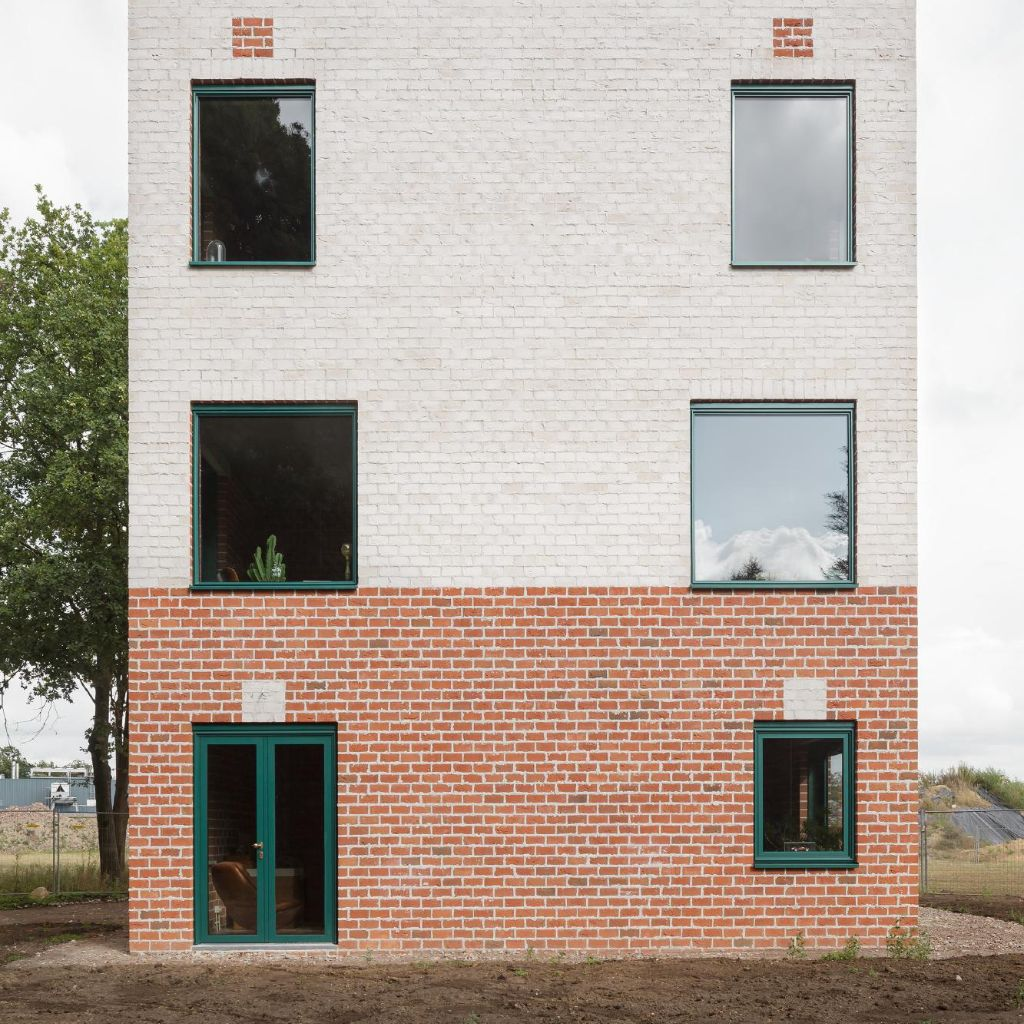
\includegraphics[width=\linewidth]{Images/LoRAs/Geleding/Training_images/6.jpg} &
      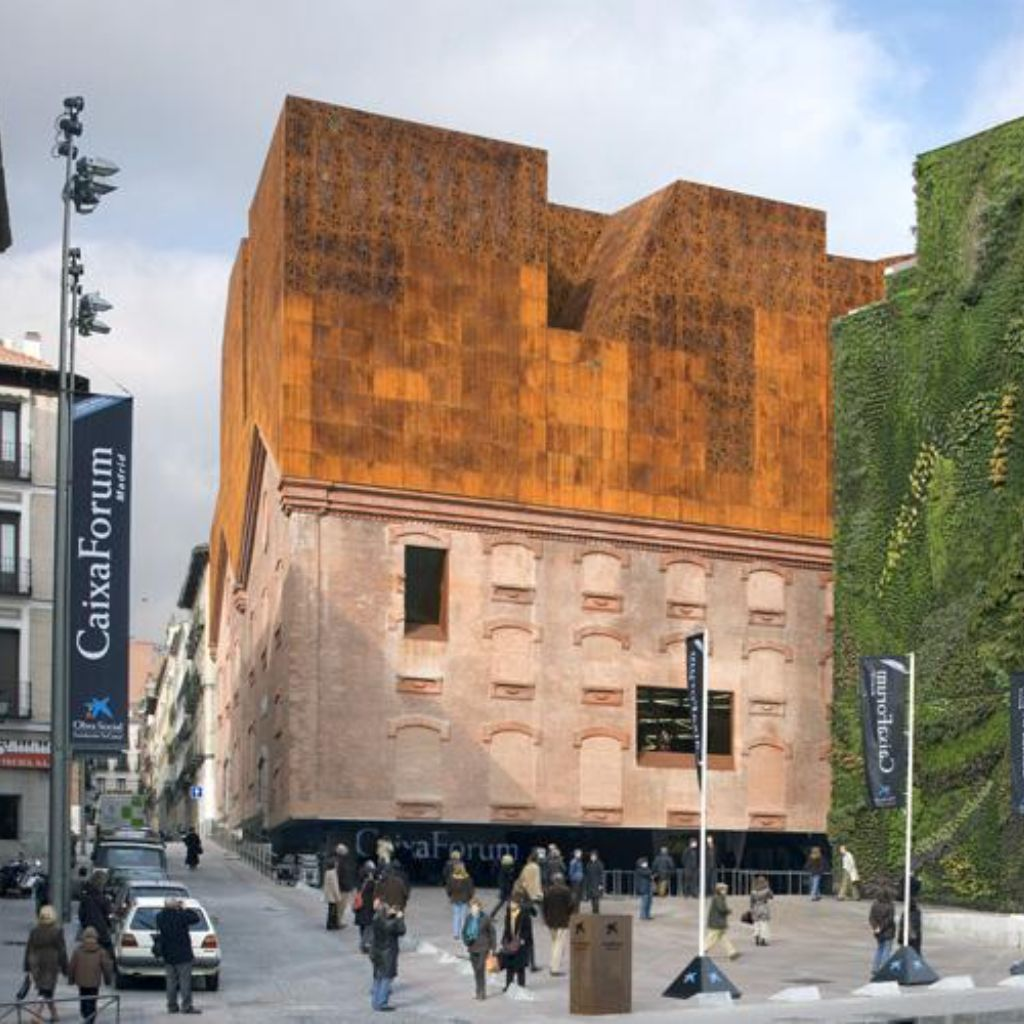
\includegraphics[width=\linewidth]{Images/LoRAs/Geleding/Training_images/7.jpg} &
      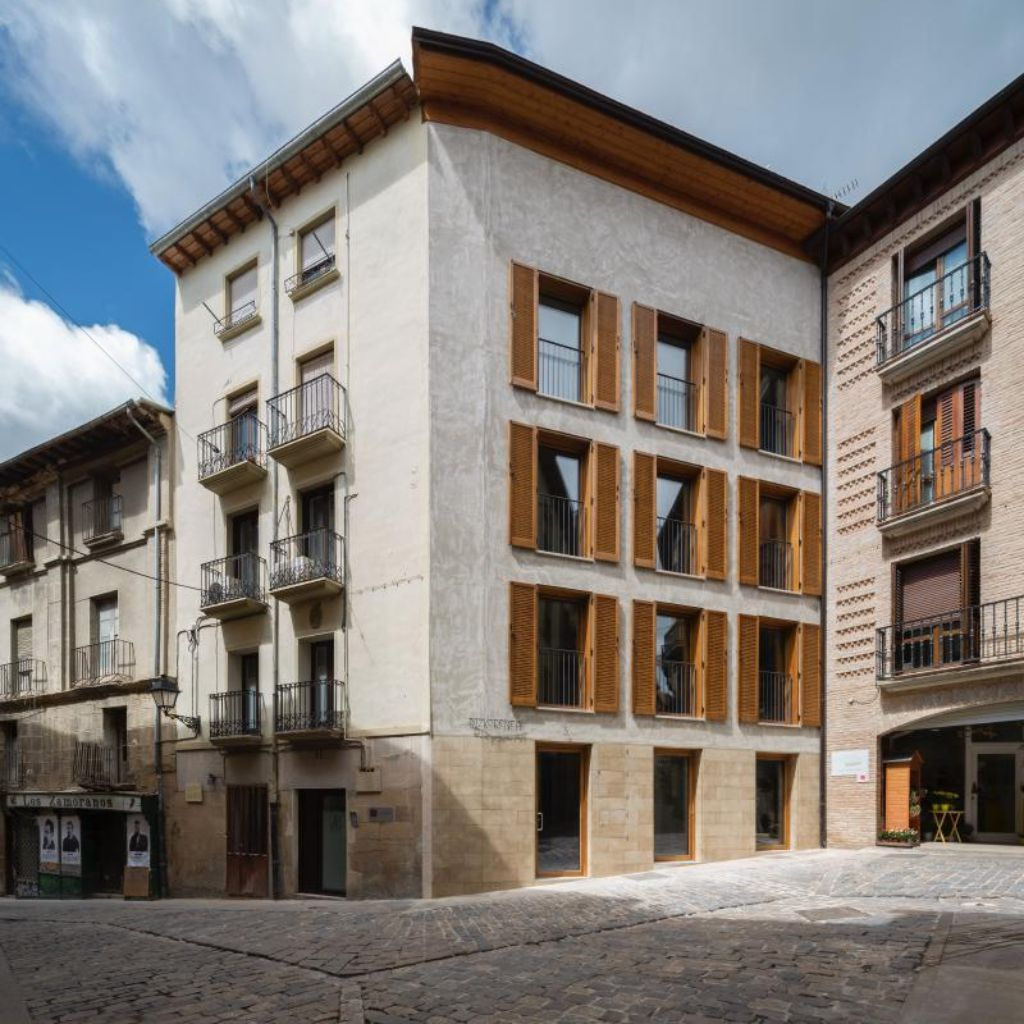
\includegraphics[width=\linewidth]{Images/LoRAs/Geleding/Training_images/8.jpg} &
      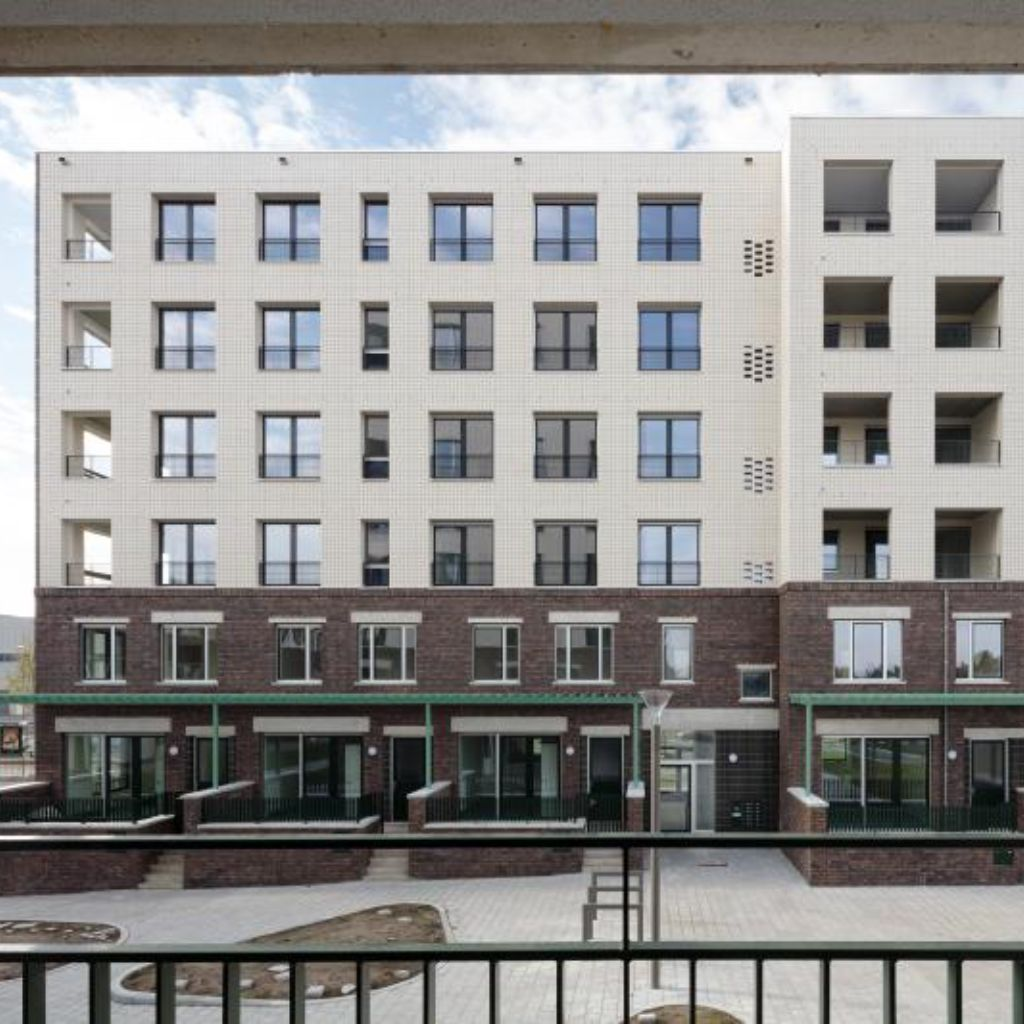
\includegraphics[width=\linewidth]{Images/LoRAs/Geleding/Training_images/9.jpg} &
      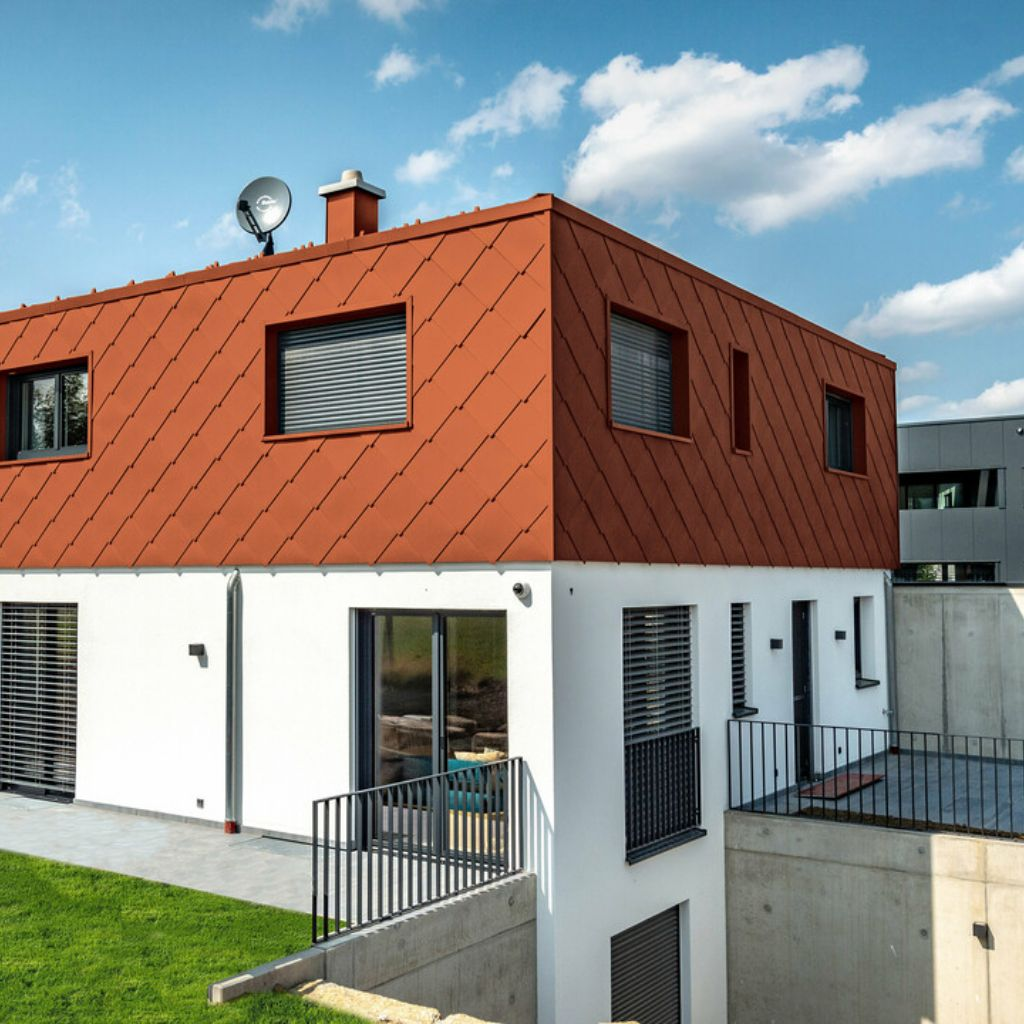
\includegraphics[width=\linewidth]{Images/LoRAs/Geleding/Training_images/10.jpg} \\[2pt]

      % Row 3: images 11–15
      \includegraphics[width=\linewidth]{Images/LoRAs/Geleding/Training_images/11.jpg} &
      \includegraphics[width=\linewidth]{Images/LoRAs/Geleding/Training_images/12.jpg} &
      \includegraphics[width=\linewidth]{Images/LoRAs/Geleding/Training_images/13.jpg} &
      \includegraphics[width=\linewidth]{Images/LoRAs/Geleding/Training_images/14.jpg} &
      \includegraphics[width=\linewidth]{Images/LoRAs/Geleding/Training_images/15.jpg} \\
    \end{tabular}%
  }
  \caption{The images used to train the geleding LoRA.}
  \label{fig:gridgeleding}
\end{figure}

\subsection{Finalized datasets for LAVA}
\subsubsection{Modulariteit}
The first LoRA for LAVA is built around modular buildings. This concept was chosen by the architect due to its contemporary relevance and its potential to enable high-quality re-use.\\
Visually, this LoRA emphasizes on generating a grid in the facade.
After validation, four images were left out of the original dataset (figure \ref{fig:removedmodulariteit}): in images 1, 3 and 4, the modularity was insufficiently clear, and in image 2 the wooden building extension felt structurally monolithic, rather than composed of modules.
\begin{figure}[H]
  \centering
   \resizebox{\textwidth}{!}{%
    \begin{tabular}{@{}cccc@{}}
      % Row 1: images 1–2
      \includegraphics[width=\linewidth]{Images/LoRAs/Modulariteit/8.jpg}&
      \includegraphics[width=\linewidth]{Images/LoRAs/Modulariteit/10.jpg}&
      \includegraphics[width=\linewidth]{Images/LoRAs/Modulariteit/12.jpeg}&
      \includegraphics[width=\linewidth]{Images/LoRAs/Modulariteit/14.jpeg}\\
    \end{tabular}
  }
  \caption{The images removed from the original modulariteit dataset.}
  \label{fig:removedmodulariteit}
\end{figure}

Figure \ref{fig:gridmodulariteit} portrays the training images for this LoRA.
\begin{figure}[H]
  \centering
  \resizebox{\textwidth}{!}{%
    \begin{tabular}{@{}ccccc@{}}
      % Row 1: images 1–5
      \includegraphics[width=\linewidth]{Images/LoRAs/Modulariteit/Training_images/1.jpg} &
      \includegraphics[width=\linewidth]{Images/LoRAs/Modulariteit/Training_images/2.jpg} &
      \includegraphics[width=\linewidth]{Images/LoRAs/Modulariteit/Training_images/3.jpeg} &
      \includegraphics[width=\linewidth]{Images/LoRAs/Modulariteit/Training_images/4.jpg} &
      \includegraphics[width=\linewidth]{Images/LoRAs/Modulariteit/Training_images/5.jpg} \\[2pt]

      % Row 2: images 6–10
      \includegraphics[width=\linewidth]{Images/LoRAs/Modulariteit/Training_images/6.jpg} &
      \includegraphics[width=\linewidth]{Images/LoRAs/Modulariteit/Training_images/7.jpg} &
      \includegraphics[width=\linewidth]{Images/LoRAs/Modulariteit/Training_images/8.jpg} &
      \includegraphics[width=\linewidth]{Images/LoRAs/Modulariteit/Training_images/9.png} &
      \includegraphics[width=\linewidth]{Images/LoRAs/Modulariteit/Training_images/10.JPG} \\[2pt]

      % Row 3: images 11–15
      \includegraphics[width=\linewidth]{Images/LoRAs/Modulariteit/Training_images/11.jpg} &
      \includegraphics[width=\linewidth]{Images/LoRAs/Modulariteit/Training_images/12.jpg} &
      \includegraphics[width=\linewidth]{Images/LoRAs/Modulariteit/Training_images/13.jpg} &
      \includegraphics[width=\linewidth]{Images/LoRAs/Modulariteit/Training_images/14.jpg} &
      \includegraphics[width=\linewidth]{Images/LoRAs/Modulariteit/Training_images/15.jpg} \\
    \end{tabular}%
  }
  \caption{The images used to train the Modulariteit LoRA.}
  \label{fig:gridmodulariteit}
\end{figure}
\subsubsection{Ghoek}
The second LoRA portrays rounded facade corners, a formal element often used in LAVA's projects.\\
After validation, two images (Figure \ref{fig:removedghoek}) were excluded from the original dataset. The first contained an excessive number of curved corners, and the second displayed a curve that was too large.
\begin{figure}[H]
  \centering
  % First image
  \includegraphics[width=0.24\textwidth]{Images/LoRAs/Ghoek/2.jpg}%
  \hspace{0.005\textwidth} % small gap; adjust if needed
  % Second image
  \includegraphics[width=0.24\textwidth]{Images/LoRAs/Ghoek/8.jpg}
  \caption{The images removed from the original Ghoek dataset.}
  \label{fig:removedghoek}
\end{figure}
Figure \ref{fig:gridghoek} portrays the training images for this LoRA.
\begin{figure}[H]
  \centering
  \resizebox{\textwidth}{!}{%
    \begin{tabular}{@{}ccccc@{}}
      % Row 1: images 1–5
      \includegraphics[width=\linewidth]{Images/LoRAs/Ghoek/Training_images/1.jpeg} &
      \includegraphics[width=\linewidth]{Images/LoRAs/Ghoek/Training_images/2.jpg} &
      \includegraphics[width=\linewidth]{Images/LoRAs/Ghoek/Training_images/3.jpg} &
      \includegraphics[width=\linewidth]{Images/LoRAs/Ghoek/Training_images/4.jpg} &
      \includegraphics[width=\linewidth]{Images/LoRAs/Ghoek/Training_images/5.jpg} \\[2pt]

      % Row 2: images 6–10
      \includegraphics[width=\linewidth]{Images/LoRAs/Ghoek/Training_images/6.jpeg} &
      \includegraphics[width=\linewidth]{Images/LoRAs/Ghoek/Training_images/7.jpeg} &
      \includegraphics[width=\linewidth]{Images/LoRAs/Ghoek/Training_images/8.jpg} &
      \includegraphics[width=\linewidth]{Images/LoRAs/Ghoek/Training_images/9.jpg} &
      \includegraphics[width=\linewidth]{Images/LoRAs/Ghoek/Training_images/10.JPG} \\[2pt]

      % Row 3: images 11–15
      \includegraphics[width=\linewidth]{Images/LoRAs/Ghoek/Training_images/11.jpg} &
      \includegraphics[width=\linewidth]{Images/LoRAs/Ghoek/Training_images/12.jpg} &
      \includegraphics[width=\linewidth]{Images/LoRAs/Ghoek/Training_images/13.jpg} &
      \makebox[0.19\textwidth]{} &
      \makebox[0.19\textwidth]{} \\
    \end{tabular}%
  }
  \caption{The images used to train the Ghoek LoRA.}
  \label{fig:gridghoek}
\end{figure}

\subsubsection{Plintwerking}
The third and final LoRA for LAVA represents a 'plinth effect', often used in contemporary architecture to differentiate the ground floor of a building from the upper levels.\\
After validation, three images (figure \ref{fig:gridplintwerking}) were removed from the original dataset. In the first and third, the only distinction between the plinth and the upper floors was materiality, which was considered insufficient; in the second, the architect judged that the building was not effectively emphasized in the image, preferring other images of the same building.
\begin{figure}[H]
  \centering
  \includegraphics[width=0.24\textwidth]{Images/LoRAs/Plintwerking/2.jpg}%
  \hspace{0.005\textwidth} 
  \includegraphics[width=0.24\textwidth]{Images/LoRAs/Plintwerking/5.jpeg}
  \hspace{0.005\textwidth}
  \includegraphics[width=0.24\textwidth]{Images/LoRAs/Plintwerking/6.jpg}
  \caption{The images removed from the original Plintwerking dataset.}
  \label{fig:removedplintwerking}
\end{figure}
Figure \ref{fig:gridplintwerking} portrays the training images for this LoRA.
\begin{figure}[H]
  \centering
  \resizebox{\textwidth}{!}{%
    \begin{tabular}{@{}ccccc@{}}
      % Row 1: images 1–5
      \includegraphics[width=\linewidth]{Images/LoRAs/Plintwerking/Training_images/1.jpg} &
      \includegraphics[width=\linewidth]{Images/LoRAs/Plintwerking/Training_images/2.jpg} &
      \includegraphics[width=\linewidth]{Images/LoRAs/Plintwerking/Training_images/3.jpg} &
      \includegraphics[width=\linewidth]{Images/LoRAs/Plintwerking/Training_images/4.jpeg} &
      \includegraphics[width=\linewidth]{Images/LoRAs/Plintwerking/Training_images/5.jpg} \\[2pt]

      % Row 2: images 6–10
      \includegraphics[width=\linewidth]{Images/LoRAs/Plintwerking/Training_images/6.jpg} &
      \includegraphics[width=\linewidth]{Images/LoRAs/Plintwerking/Training_images/7.jpeg} &
      \includegraphics[width=\linewidth]{Images/LoRAs/Plintwerking/Training_images/8.jpeg} &
      \includegraphics[width=\linewidth]{Images/LoRAs/Plintwerking/Training_images/9.jpg} &
      \includegraphics[width=\linewidth]{Images/LoRAs/Plintwerking/Training_images/10.jpg} \\[2pt]

      % Row 3: images 11–12 (plus empty placeholders)
      \includegraphics[width=\linewidth]{Images/LoRAs/Plintwerking/Training_images/11.jpg} &
      \includegraphics[width=\linewidth]{Images/LoRAs/Plintwerking/Training_images/12.jpg} &
      \makebox[0.19\textwidth]{} &
      \makebox[0.19\textwidth]{} &
      \makebox[0.19\textwidth]{} \\
    \end{tabular}%
  }
  \caption{The images used to train the Plintwerking LoRA.}
  \label{fig:gridplintwerking}
\end{figure}
\subsection{Conclusion}
The training datasets for each LoRA were assembled through a workflow of image collection, resizing, and validation by the architects themselves. \\
Initial datasets of 15–19 images per concept were rated by the architects on a 3-point likert scale, which led to the removal of images that poorly illustrated the target feature, whether due to misleading textures, inadequate composition, or stylistic mismatch.

Across the six LoRAs, the finalized image sets contain between 12 and 15 images each. Every retained image clearly exemplifies its respective concept under varied lighting, scale, and perspective conditions. This selection protocol provides high-quality, concept-specific training data.

\newpage
\section{LoRA training methodology}\label{sec:LoRA training methodology}
To train LoRA models on the finalized image datasets, a methodology was developed over the course of several months of experimentation. To train the LoRAs, a cloud service called Replicate (\href{https://replicate.com/}{replicate.com}) was used.\\
Figure \ref{fig:lora-methodology} shows the process of training the LoRA models. This process is iterative; thus, there are multiple versions that each LoRA goes through until it's a finished product.
\begin{figure}[H]
    \centering
    \includegraphics[width=\linewidth]{Images//Methodology/LoRA methodology.jpg}
    \caption{The methodology used to train each of the 6 LoRA models.}
    \label{fig:lora-methodology}
\end{figure}

\subsection{Image captioning}
To guide LoRA training toward learning the target concept, all images were captioned with the custom GPT 'LoRA prompt generator' (section \ref{sec:ChatGPT}). This ensured that the training captions always had the same structure as the prompts used to generate output images.\\
\\
Refining the captions iteratively is essential, because output images of initial versions of the LoRA rarely show satisfactory results. Only after training and evaluating the first versions of the LoRA, one can identify where the LoRA lays its focus the most and modify the captions accordingly. Two frequent problems occuring here are 'overfitting', which happens when the LoRA associates irrelevant details with the concept, and 'underfitting', which happens when the captions are not clear enough and the LoRA does not grasp the concept. Only after some repetitions of captioning, training and testing, the LoRA grasps the concept in the envisioned way.

\subsection{LoRA training}
After a ZIP-file containing all the images and all the captions was created, Ostris' \href{https://replicate.com/ostris/flux-dev-lora-trainer/train}{FLUX.1 [dev] LoRA trainer} on replicate.com was used. This model is based on Ostris' public GitHub-repository 'ai-toolkit' (the repository can be found on \href{https://github.com/ostris/ai-toolkit}{https://github.com/ostris/ai-toolkit}).\\
In the form on the website, the trigger word of the LoRA has to be entered, as well as the amount of steps to train and the lora rank. For all the LoRAs, the steps were kept to the default number of 1000 and the lora rank was kept to 16, concentrating on improving the captions when iterating versions.

\subsection{LoRA testing}
To test the LoRA models, the researcher generated images using the custom ComfyUI workflow and the custom GPT, assessing the LoRA models in several contexts and use cases. After generating numerous images and critically reviewing them, the researcher gets an idea for what the LoRA might improve upon.\\
After testing the LoRA, if the quality is not satisfactory, the researcher went back to the first step of captioning the images and training a new version of the LoRA, after which the cycle repeats.

\subsection{Finalized LoRA}
The LoRA models were finalized when the researcher was satisfied with the generated output images.

\section{Evaluation sessions} \label{sec:Evaluation sessions}
To research how the trained LoRA models could help Flemish architects design, images generated with the LoRA models were evaluated by professional Flemish architects in experimental design phases. 
\subsection{Participants}
For this study, two architectural offices participated, which are both originated in Leuven: DMOA and LAVA. One partner from each office participated in the study. 

\subsection{Structure of the sessions}
\begin{figure}[H]
    \centering
    \includegraphics[width=1\linewidth]{Images/Methodology/timeline_evaluation_sessions.jpg}
    \caption{The chronological structure of the evaluation sessions.}
    \label{fig:timeline}
\end{figure}
Figure \ref{fig:timeline} portrays the structure of the evaluation sessions, which consisted of 2 segments where images were evaluated: a structured segment and an unstructured segment.\\
The \textbf{structured segment} was divided into 3 design phases: sketch design, preliminary design, and presentation (\cite{riba_riba_2024}, part 1 chapter 1). To keep the start of these phases equal for both architects, each phase starts from a new small design brief.\\
After the structured segment, the researcher conducted a brief \textbf{interview} with the participating architects, during which they reflected on the AI-generated images.\\
This was followed by the \textbf{unstructured segment}, in which the LoRA models were applied to images provided by the architects themselves, allowing for an exploration of how the LoRA models perform when integrated into their own design projects.\\~\\
The sketch design and preliminary design phases are focused on \textbf{Text-to-Image generation}, while the presentation phase and unstructured segment are focused on \textbf{Image-to-Image generation} using ControlNet.\\
Each of the phases is explained in more detail in the following sections.
\subsubsection{Sketch design}
For the sketch design phase, the design brief concerned an apartment building  located near a public park in Brussels (figure \ref{fig:sketch-site}), containing public functions (such as stores or workshop spaces) on the ground floor.\\
In this phase, the architects were told to focus on the \textbf{volumetry} of the building.
\begin{figure}[H]
    \centering
    \includegraphics[width=0.75\linewidth]{Images/Methodology/Sketch_design_brief.png}
    \caption{The site for the sketch design phase.}
    \label{fig:sketch-site}
\end{figure}

\subsubsection{Preliminary design}
In the preliminary design phase, the idea is that the volume is already determined; thus, the volumetry for this phase was predetermined by the researcher: a cubic volume. The architects were told to shift their focus to concepts like materiality, composition and execution of the facade.\\
The brief for this phase was to design a freestanding family home for a family of 2 parents and 2 children. \\
\begin{figure}
    \centering
    \includegraphics[width=0.75\linewidth]{Images/Methodology/Preliminary_design_brief.png}
    \caption{The site for the preliminary design phase.}
    \label{fig:preliminary-site}
\end{figure}

\subsection{Presentation}
The presentation phase simulated the stage in architectural design where a presentation has to be held for clients. Since the design would already be finished when starting this phase, images were generated based on the geometry of a 3D-model (figure \ref{fig:presentation-image}) using ControlNet with a Canny preprocessor.
\begin{figure}[H]
    \centering
    \includegraphics[width=0.5\linewidth]{Images//Methodology/presentation_image.png}
    \caption{The image that served as a base for the generated images in the Presentation design phase.}
    \label{fig:presentation-image}
\end{figure}

\subsection{Data collection}
The following data were collected for each participating architect:
\begin{itemize}
    \item Screen and audio recordings of the sessions; 
    \item Video recordings of the sessions.
\end{itemize}

Both sessions were thematically analyzed by the researcher.